\documentclass[11pt,edeposit,draftthesis]{uiucthesis2020}

% {{{ packages

\usepackage{blindtext}

% math
\usepackage{fixmath}
\usepackage{amsmath}
\usepackage{amsthm}
\usepackage{amssymb}
\usepackage{stmaryrd}

% pretty links
\usepackage{xparse}
\usepackage{hyperref}
\usepackage{cleveref}
\usepackage{graphicx}
\hypersetup{
    colorlinks=true,
    urlcolor=blue,
    citecolor=black,
    linkcolor=black
}

% better environments
\usepackage[shortlabels]{enumitem}
\usepackage{booktabs}

% fancier font
\usepackage[sc]{mathpazo}
% better typography
\usepackage[activate={true,nocompatibility}, % activate protrusion and font expansion
            final,              % enable microtype, use draft to disable
            tracking=true,
            kerning=true,       % optimise interactions between characters
            spacing=true,       % more uniform spacing between words
            factor=1100,        % more protrusion
            stretch=10,         % smaller values (default 20, 20) to avoid blurring
            shrink=10]{microtype}
\microtypecontext{spacing=nonfrench}
\SetTracking{encoding={*}, shape=sc}{40}

% }}}

% {{{ commands

\NewDocumentCommand \dx { O{x} } {\,\mathrm{d} #1}
\NewDocumentCommand \vect { m } { \mathbold{#1} }
\NewDocumentCommand \jump { m } { \left\llbracket #1 \right\rrbracket }
\NewDocumentCommand \avg { m } { \left\langle #1 \right\rangle}
\NewDocumentCommand \od { m m } { \dfrac{\mathrm{d} #1}{\mathrm{d} #2} }
\NewDocumentCommand \pd { m m } { \dfrac{\partial #1}{\partial #2} }

% }}}

% {{{ title

\title{Magnetic ordering and spin wave dynamics in transition metal arsenides}
\author{Manohar H. Karigerasi}
\department{Materials Science and Engineering}

\schools{
B. Tech., Indian Institute of Technology Roorkee, 2016 \\
M. S., University of Illinois at Urbana-Champaign, 2017
}

\phdthesis
\advisor{Daniel P. Shoemaker}
\degreeyear{2021}

\committee{
Associate Professor Daniel P. Shoemaker, Chair \\
Professor David G. Cahill \\
Professor Jian-Min Zuo \\
Research Assistant Professor Gregory MacDougall \\
}

% }}}

\begin{document}

\maketitle

% {{{ front matter

\begin{frontmatter}

\begin{abstract}


Metallic antiferromagnets have gained interest in recent times due to the possibility of being useful as a memory device. Arsenic forms a large pool of magnetic metals in combination with other transition metals that have largely been ignored so far. In this report, we discover a new ternary metallic arsenide in the Cu-Mn-As phase space, identify its chemical and magnetic structure, and characterize its electrical and magnetic properties. We also carry out the magnetic structure refinement of Mn$_3$As$_2$ from neutron powder diffraction data at different temperatures to understand the magnetic ordering in Mn-As compounds. Using inelastic neutron scattering measurements, we determine exchange interactions in Fe$_2$As, which has the same structure as CuMnAs, showing a highly 2D magnon character although the phonons are 3D. Finally, we report a magnetic-structural coupled transition across 300 K in tetragonal CuMnAs and determine the correct magnetic structure of the compound.
\end{abstract}

\chapter*{Acknowledgments}

This project would not be possible without many people. Firstly, thanks to my advisor, Prof. Daniel P. Shoemaker.

%\begin{dedication}
%To Coffee
%\end{dedication}

\tableofcontents
\listoftables
\listoffigures

\end{frontmatter}

% }}}

% {{{ main matter

\begin{mainmatter}

%chapter 1
\chapter{Introduction}
Here is the first image.


\begin{figure}
\centering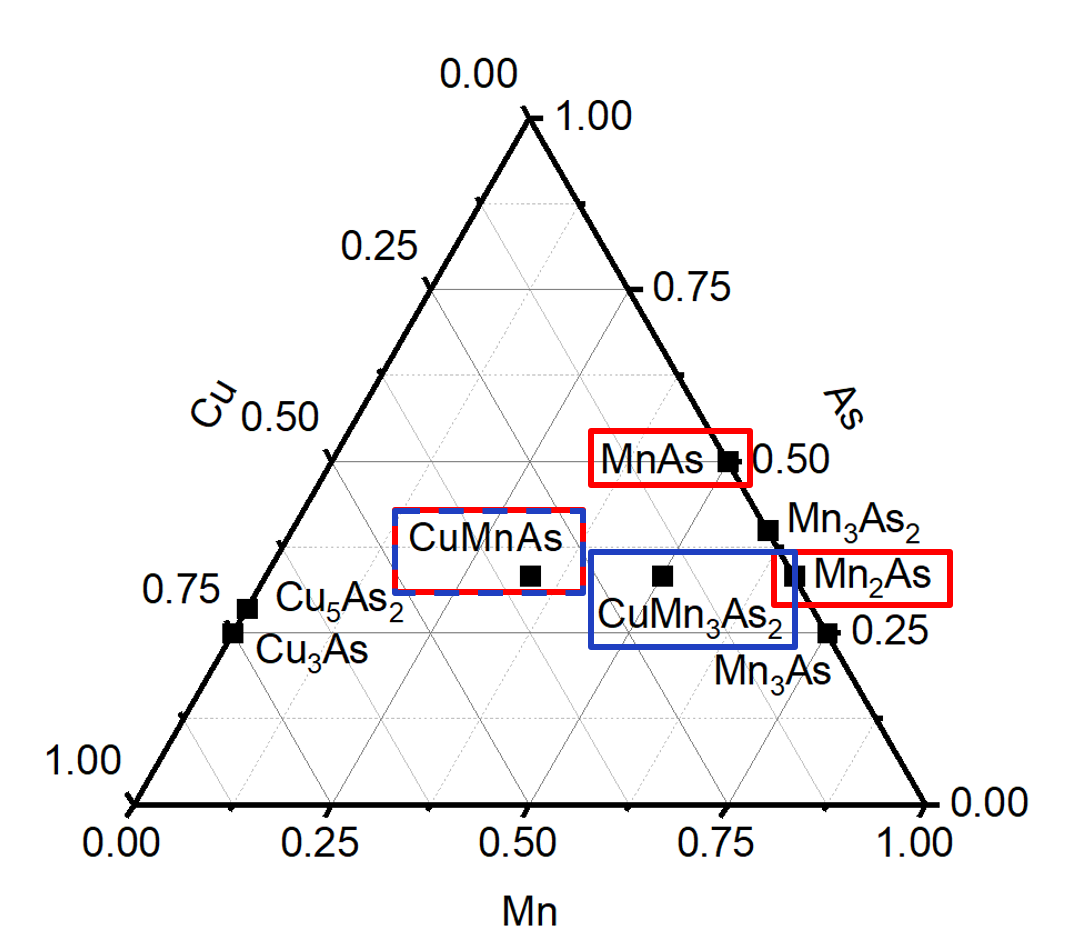
\includegraphics[width=0.8\columnwidth]{figures/ch1/Cu-Mn-As phase diagram.png} \\
\caption{\label{fig:Cu-Mn-As}
Electronic band structure
}
\end{figure}

\begin{figure}
\centering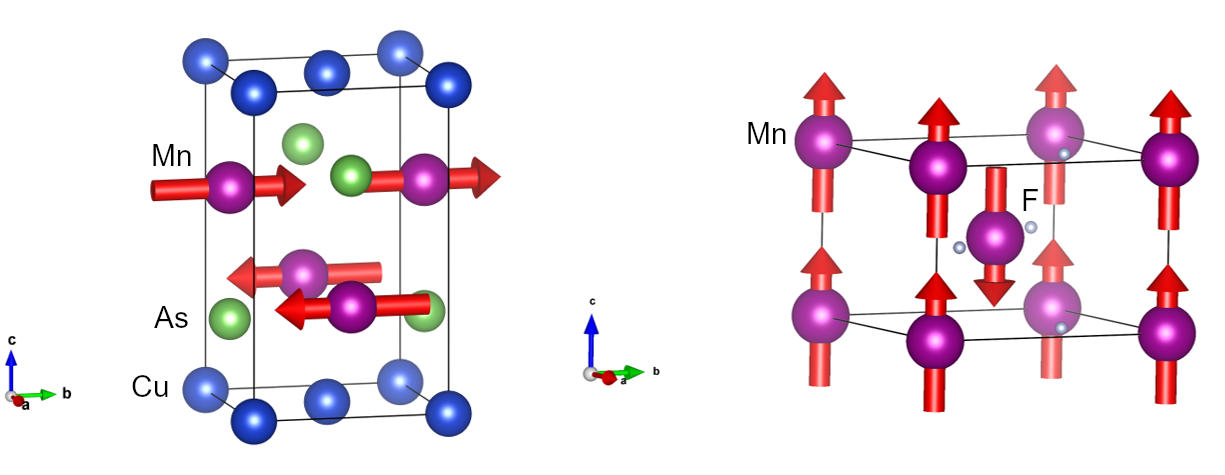
\includegraphics[width=\columnwidth]{figures/ch1/CuMnAs-MnF2.png} \\
\caption{\label{fig:tet-CuMnAs}
Electronic band structure
}
\end{figure}


\begin{figure}
\centering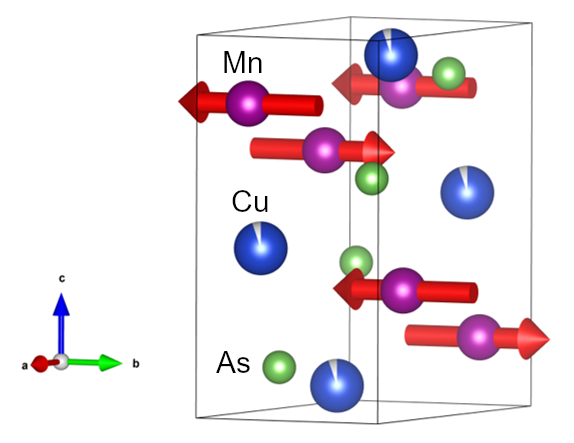
\includegraphics[width=0.5\columnwidth]{figures/ch1/ort-CuMnAs.png} \\
\caption{\label{fig:ort-CuMnAs}
Electronic band structure
}
\end{figure}




%chapter 2
\chapter{Theory of electrical switching in metallic antiferromagnets}

\begin{figure}
\centering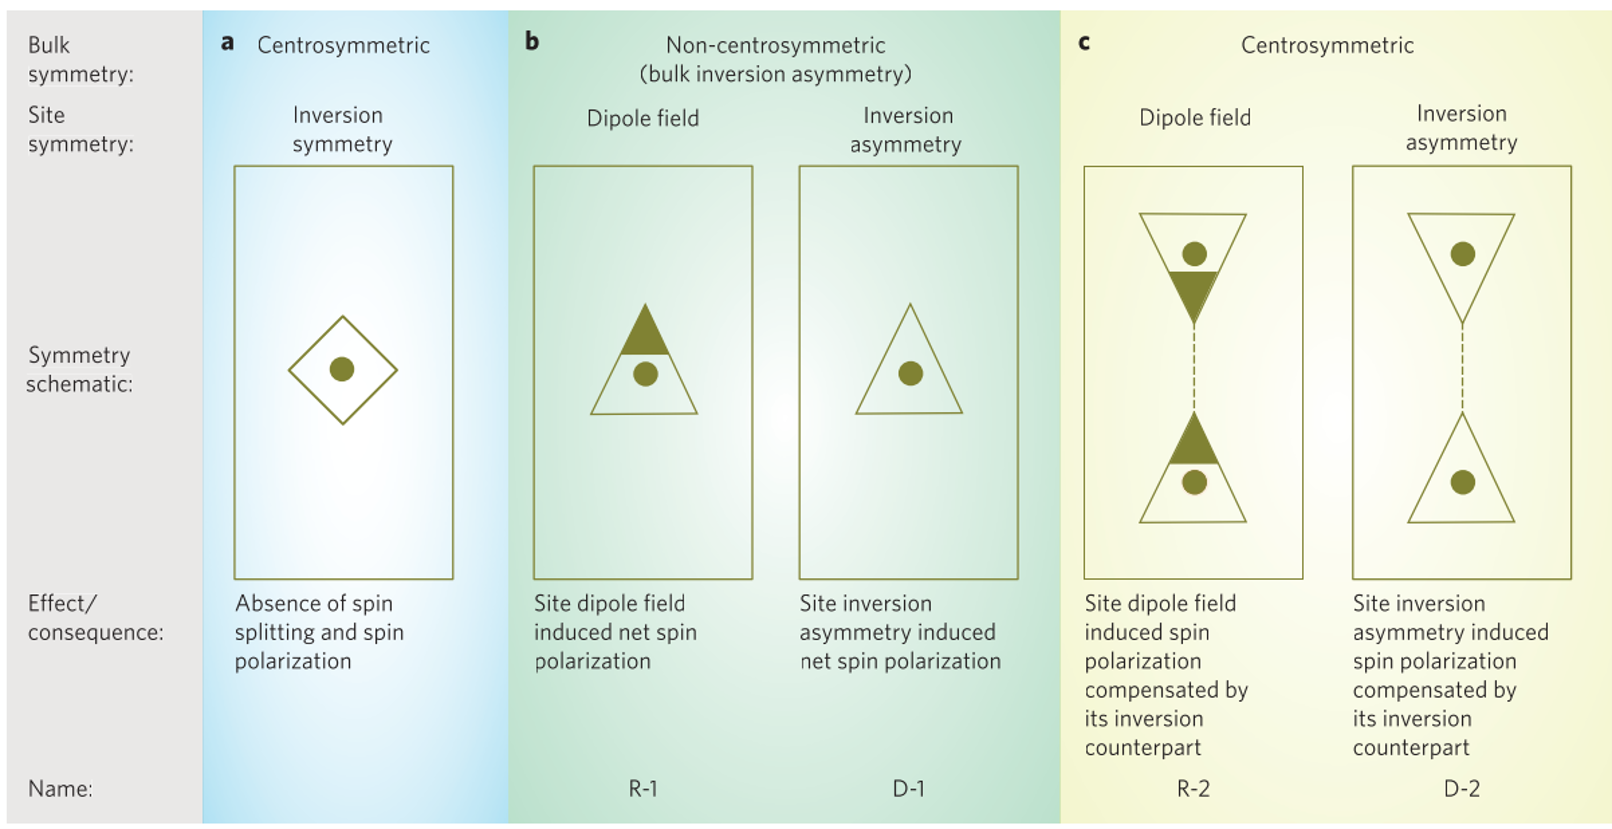
\includegraphics[width=\columnwidth]{figures/ch2/zhang_1.png} \\
\caption{\label{fig:zhang_1}
Electronic band structure
}
\end{figure}

\begin{figure}
\centering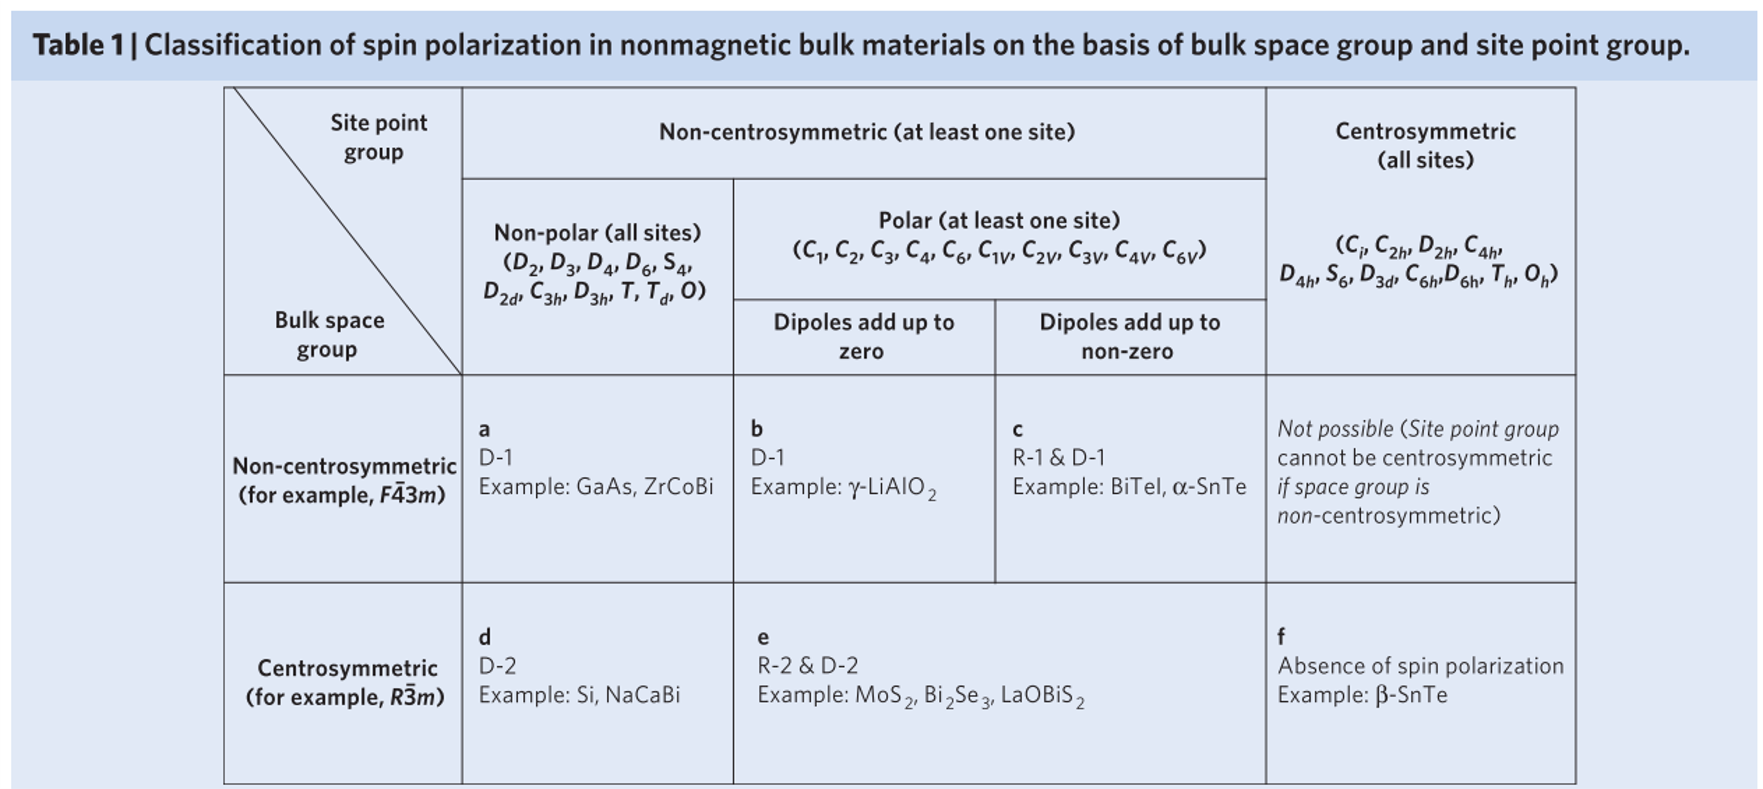
\includegraphics[width=\columnwidth]{figures/ch2/zhang_2.png} \\
\caption{\label{fig:zhang_2}
Electronic band structure
}
\end{figure}

\begin{figure}
\centering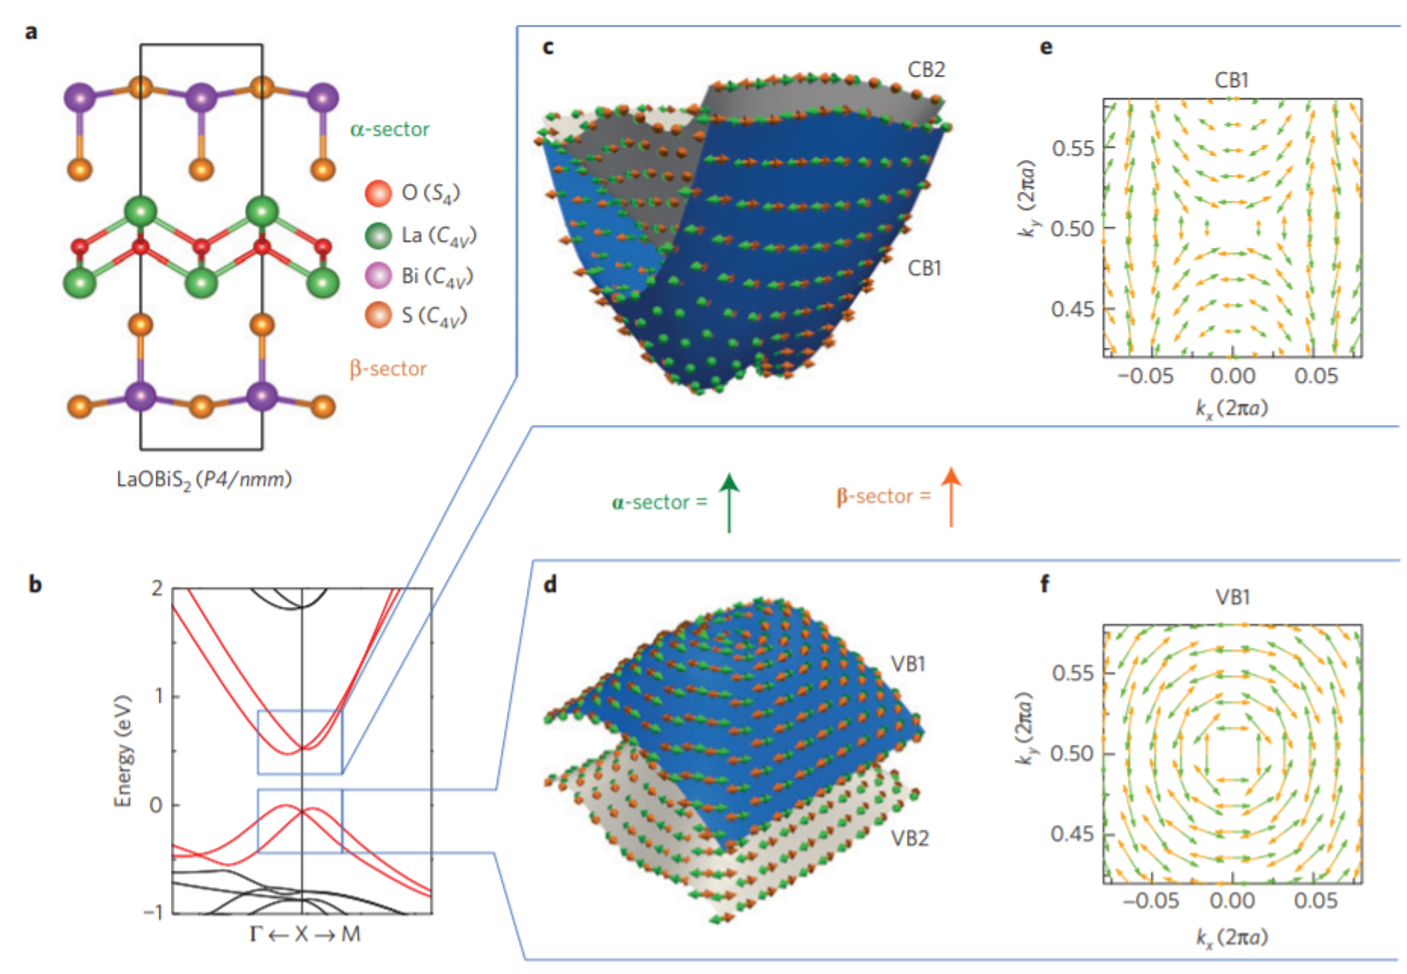
\includegraphics[width=\columnwidth]{figures/ch2/zhang_3.png} \\
\caption{\label{fig:zhang_3}
Electronic band structure
}
\end{figure}

\begin{figure}
\centering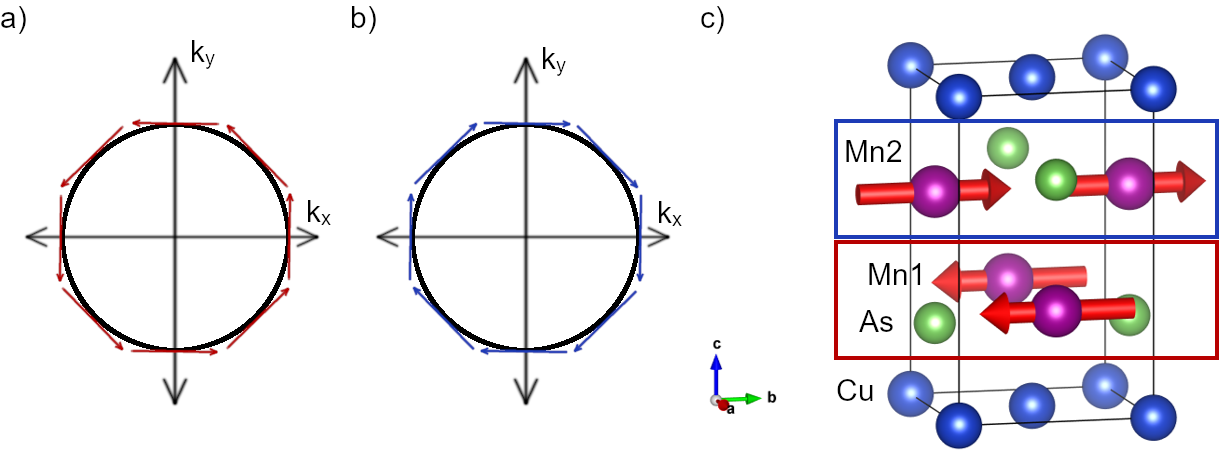
\includegraphics[width=\columnwidth]{figures/ch2/wadley_1.png} \\
\caption{\label{fig:wadley_1}
Electronic band structure
}
\end{figure}

\begin{figure}
\centering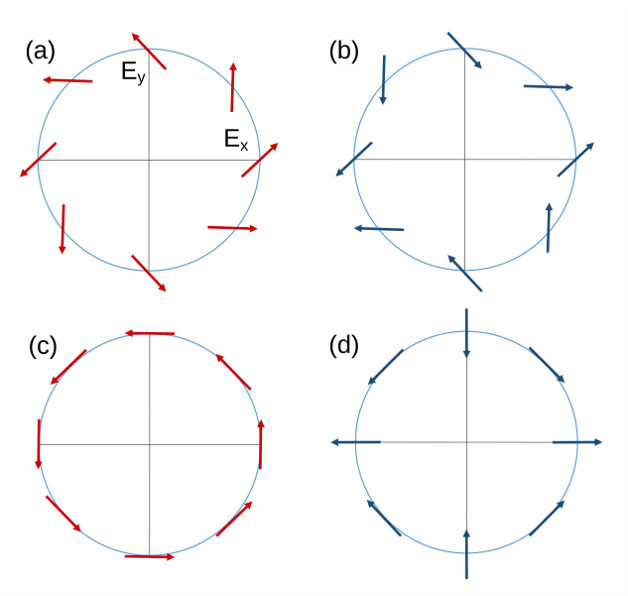
\includegraphics[width=0.7\columnwidth]{figures/ch2/rashba_dresselhaus.png} \\
\caption{\label{fig:rashba_dresselhaus}
Electronic band structure
}
\end{figure}

\begin{figure}
\centering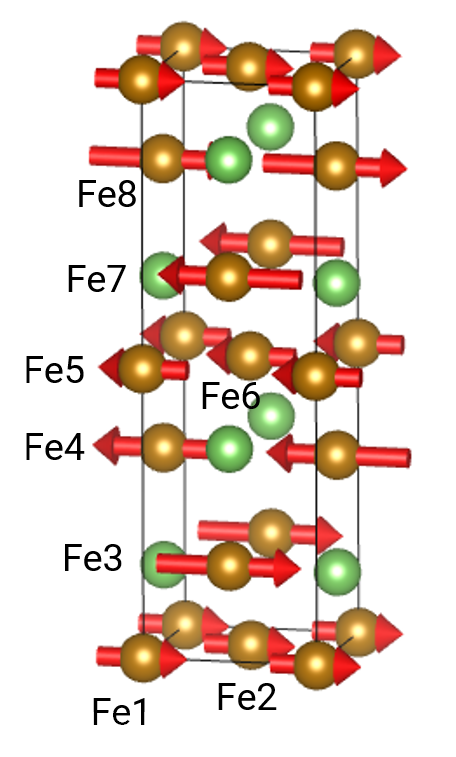
\includegraphics[width=0.3\columnwidth]{figures/ch2/Fe2As.png} \\
\caption{\label{fig:Fe2As}
Electronic band structure
}
\end{figure}

\begin{figure}
\centering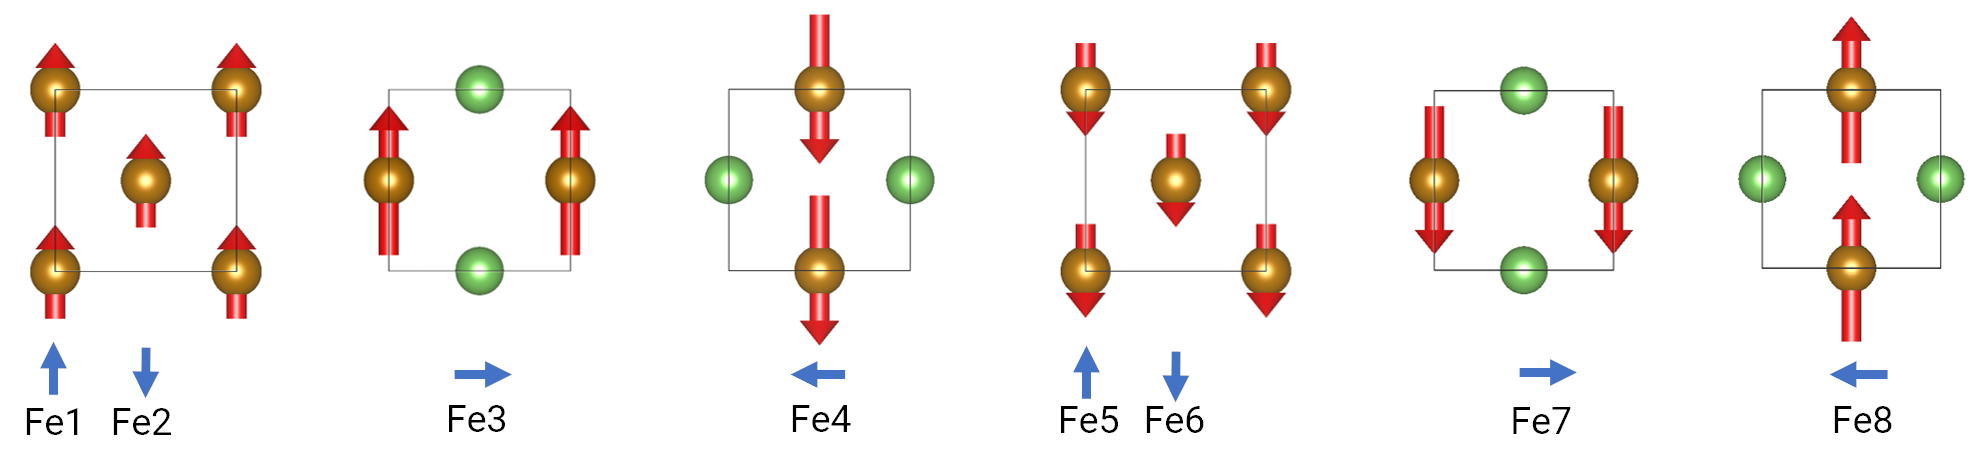
\includegraphics[width=\columnwidth]{figures/ch2/fieldlike_torque_Fe2As.png} \\
\caption{\label{fig:fieldlike_torque_Fe2As}
Electronic band structure
}
\end{figure}

\begin{figure}
\centering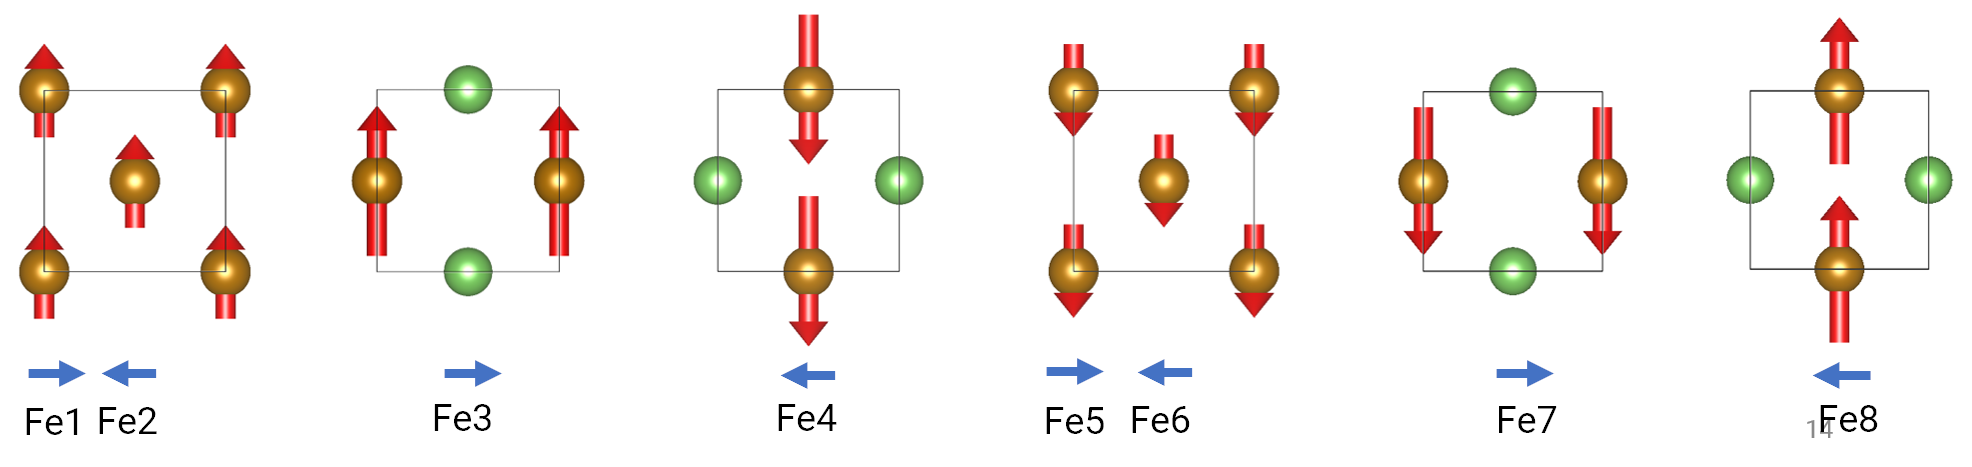
\includegraphics[width=\columnwidth]{figures/ch2/antidamping_torque_Fe2As.png} \\
\caption{\label{fig:antidamping_torque_Fe2As}
Electronic band structure
}
\end{figure}

\Blindtext[6]

%chapter 3
\chapter{Magnetic structure refinement from neutron diffraction measurements}

\begin{figure}
\centering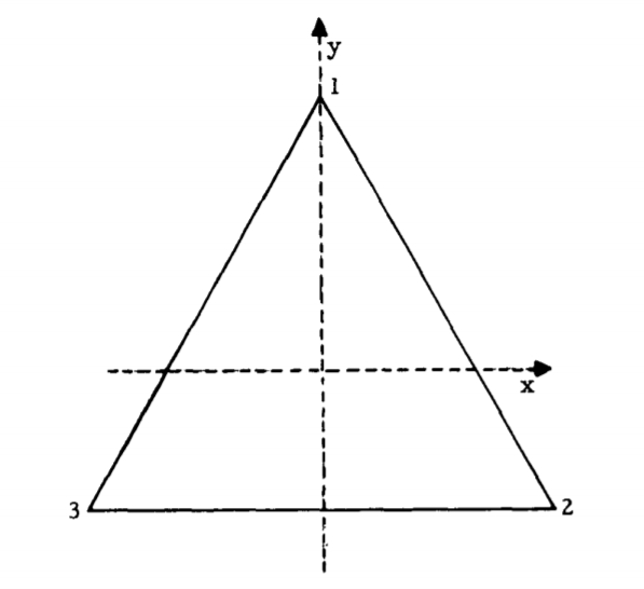
\includegraphics[width=0.5\columnwidth]{figures/ch3/C3v.png} \\
\caption{\label{fig:C3v}
Electronic band structure
}
\end{figure}

\begin{figure}
\centering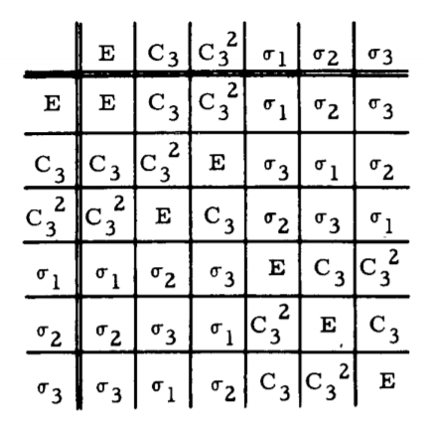
\includegraphics[width=0.5\columnwidth]{figures/ch3/group_multiplication_table_C3v.png} \\
\caption{\label{fig:gmt_C3v}
Electronic band structure
}
\end{figure}

\begin{figure}
\centering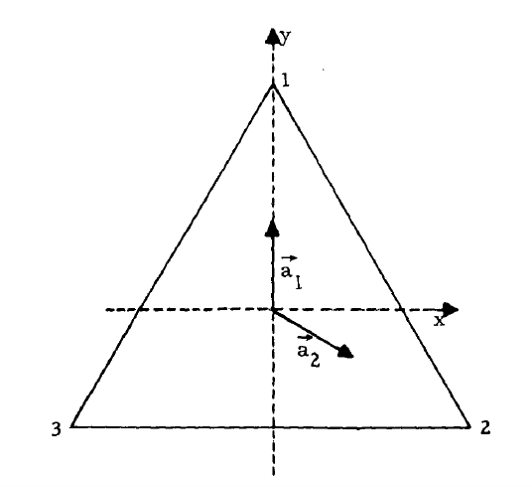
\includegraphics[width=0.5\columnwidth]{figures/ch3/C3v_a1_a2.png} \\
\caption{\label{fig:C3v_a1_a2}
Electronic band structure
}
\end{figure}

\begin{figure}
\centering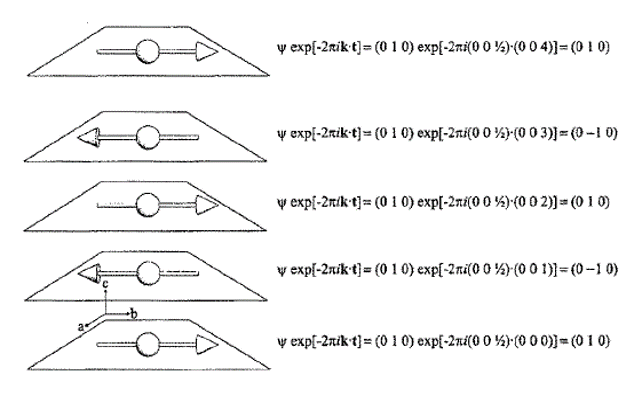
\includegraphics[width=\columnwidth]{figures/ch3/propagation_vector.png} \\
\caption{\label{fig:propagation_vector}
Electronic band structure
}
\end{figure}

\begin{figure}
\centering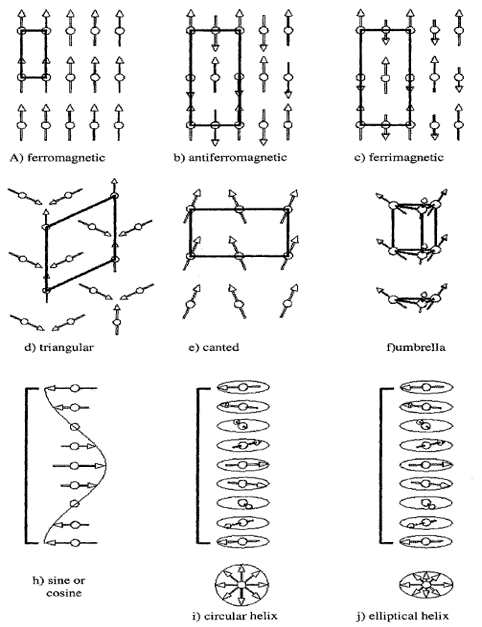
\includegraphics[width=\columnwidth]{figures/ch3/mag_structures_single_k.png} \\
\caption{\label{fig:mag_structures_single_k}
Electronic band structure
}
\end{figure}

\begin{figure}
\centering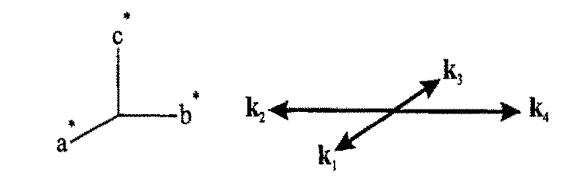
\includegraphics[width=0.7\columnwidth]{figures/ch3/star_of_propagation_vector_k.png} \\
\caption{\label{fig:star}
Electronic band structure
}
\end{figure}

\begin{figure}
\centering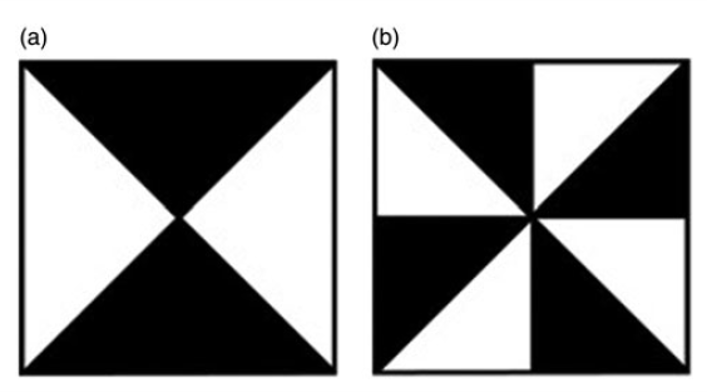
\includegraphics[width=0.5\columnwidth]{figures/ch3/symmetry_based_analysis.png} \\
\caption{\label{fig:symmetry_based_analysis}
Electronic band structure
}
\end{figure}

\Blindtext[6]

%chapter 4
\chapter{Materials synthesis and characterization}

This is a citation to~\cite{Walker2015} and~\cite{Hager2006}.

\begin{figure}
\centering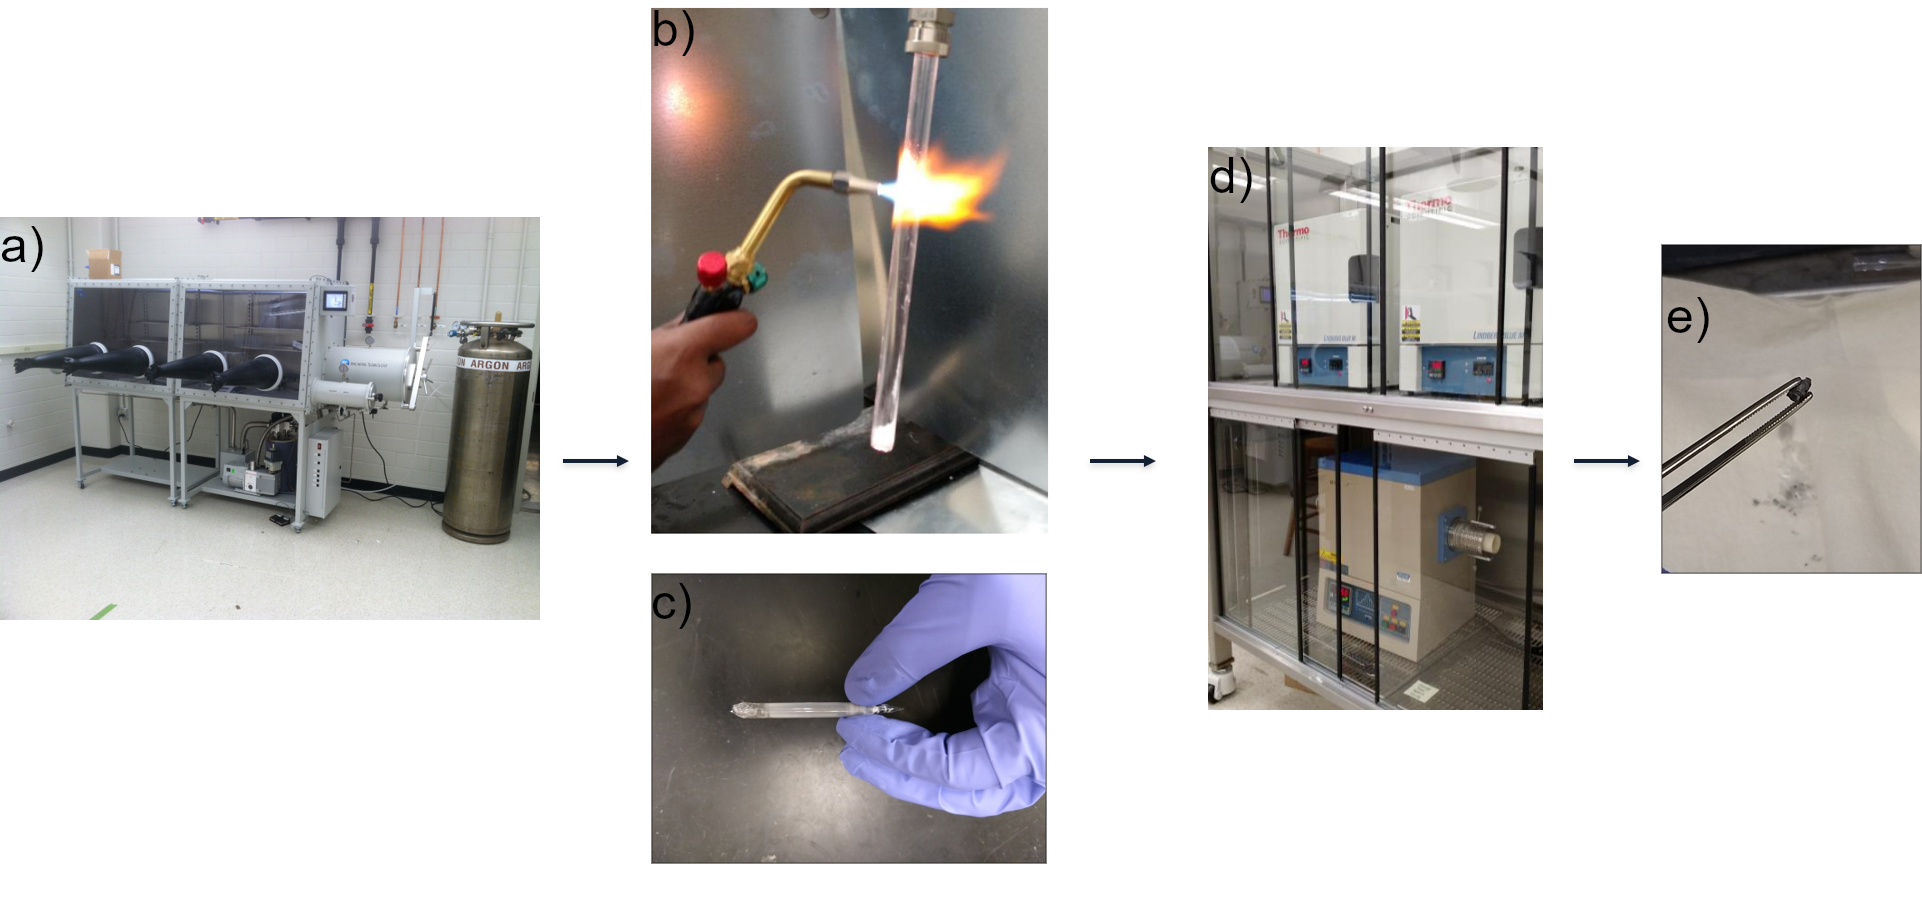
\includegraphics[width=\columnwidth]{figures/ch4/synthesis_procedure.png} \\
\caption{\label{fig:synthesis_procedure}
Electronic band structure
}
\end{figure}

%chapter 5
\chapter{Discovery and magnetic frustration of hexagonal Cu$_{0.82}$Mn$_{1.18}$As}

\begin{figure}
\centering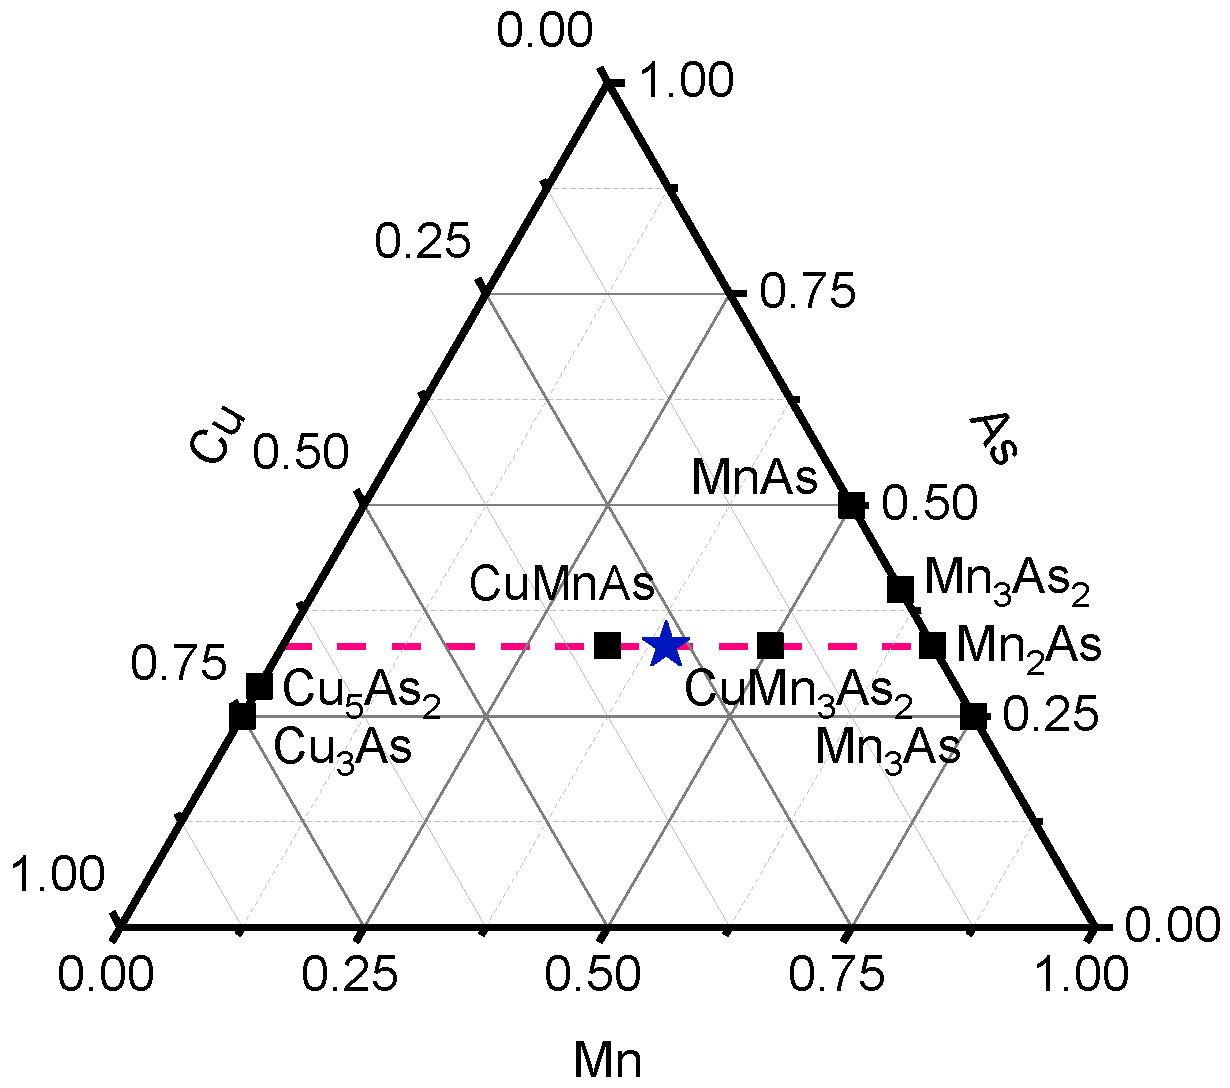
\includegraphics[width=\columnwidth]{figures/ch5/phase_diagram_cropped.pdf} \\
\caption{\label{fig:phase_diagram}
Electronic band structure
}
\end{figure}

\begin{figure}
\centering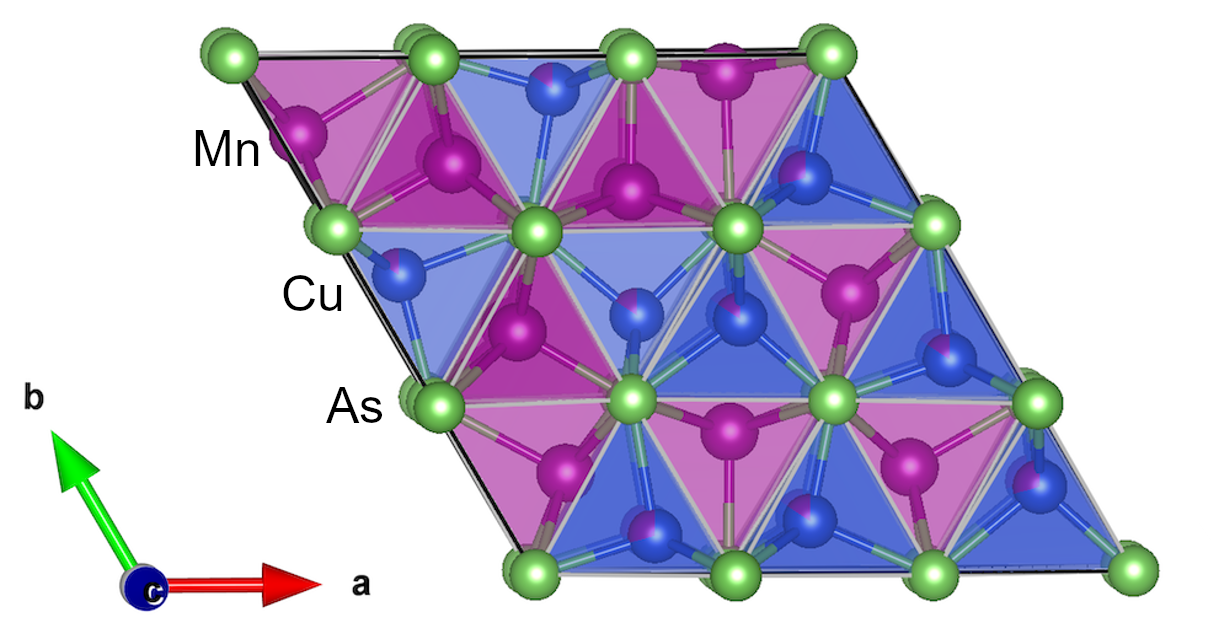
\includegraphics[width=\columnwidth]{figures/ch5/CuMnAs_chemical_structure.png} \\
\caption{\label{fig:chemical_structure}
Electronic band structure
}
\end{figure}

\begin{figure}
\centering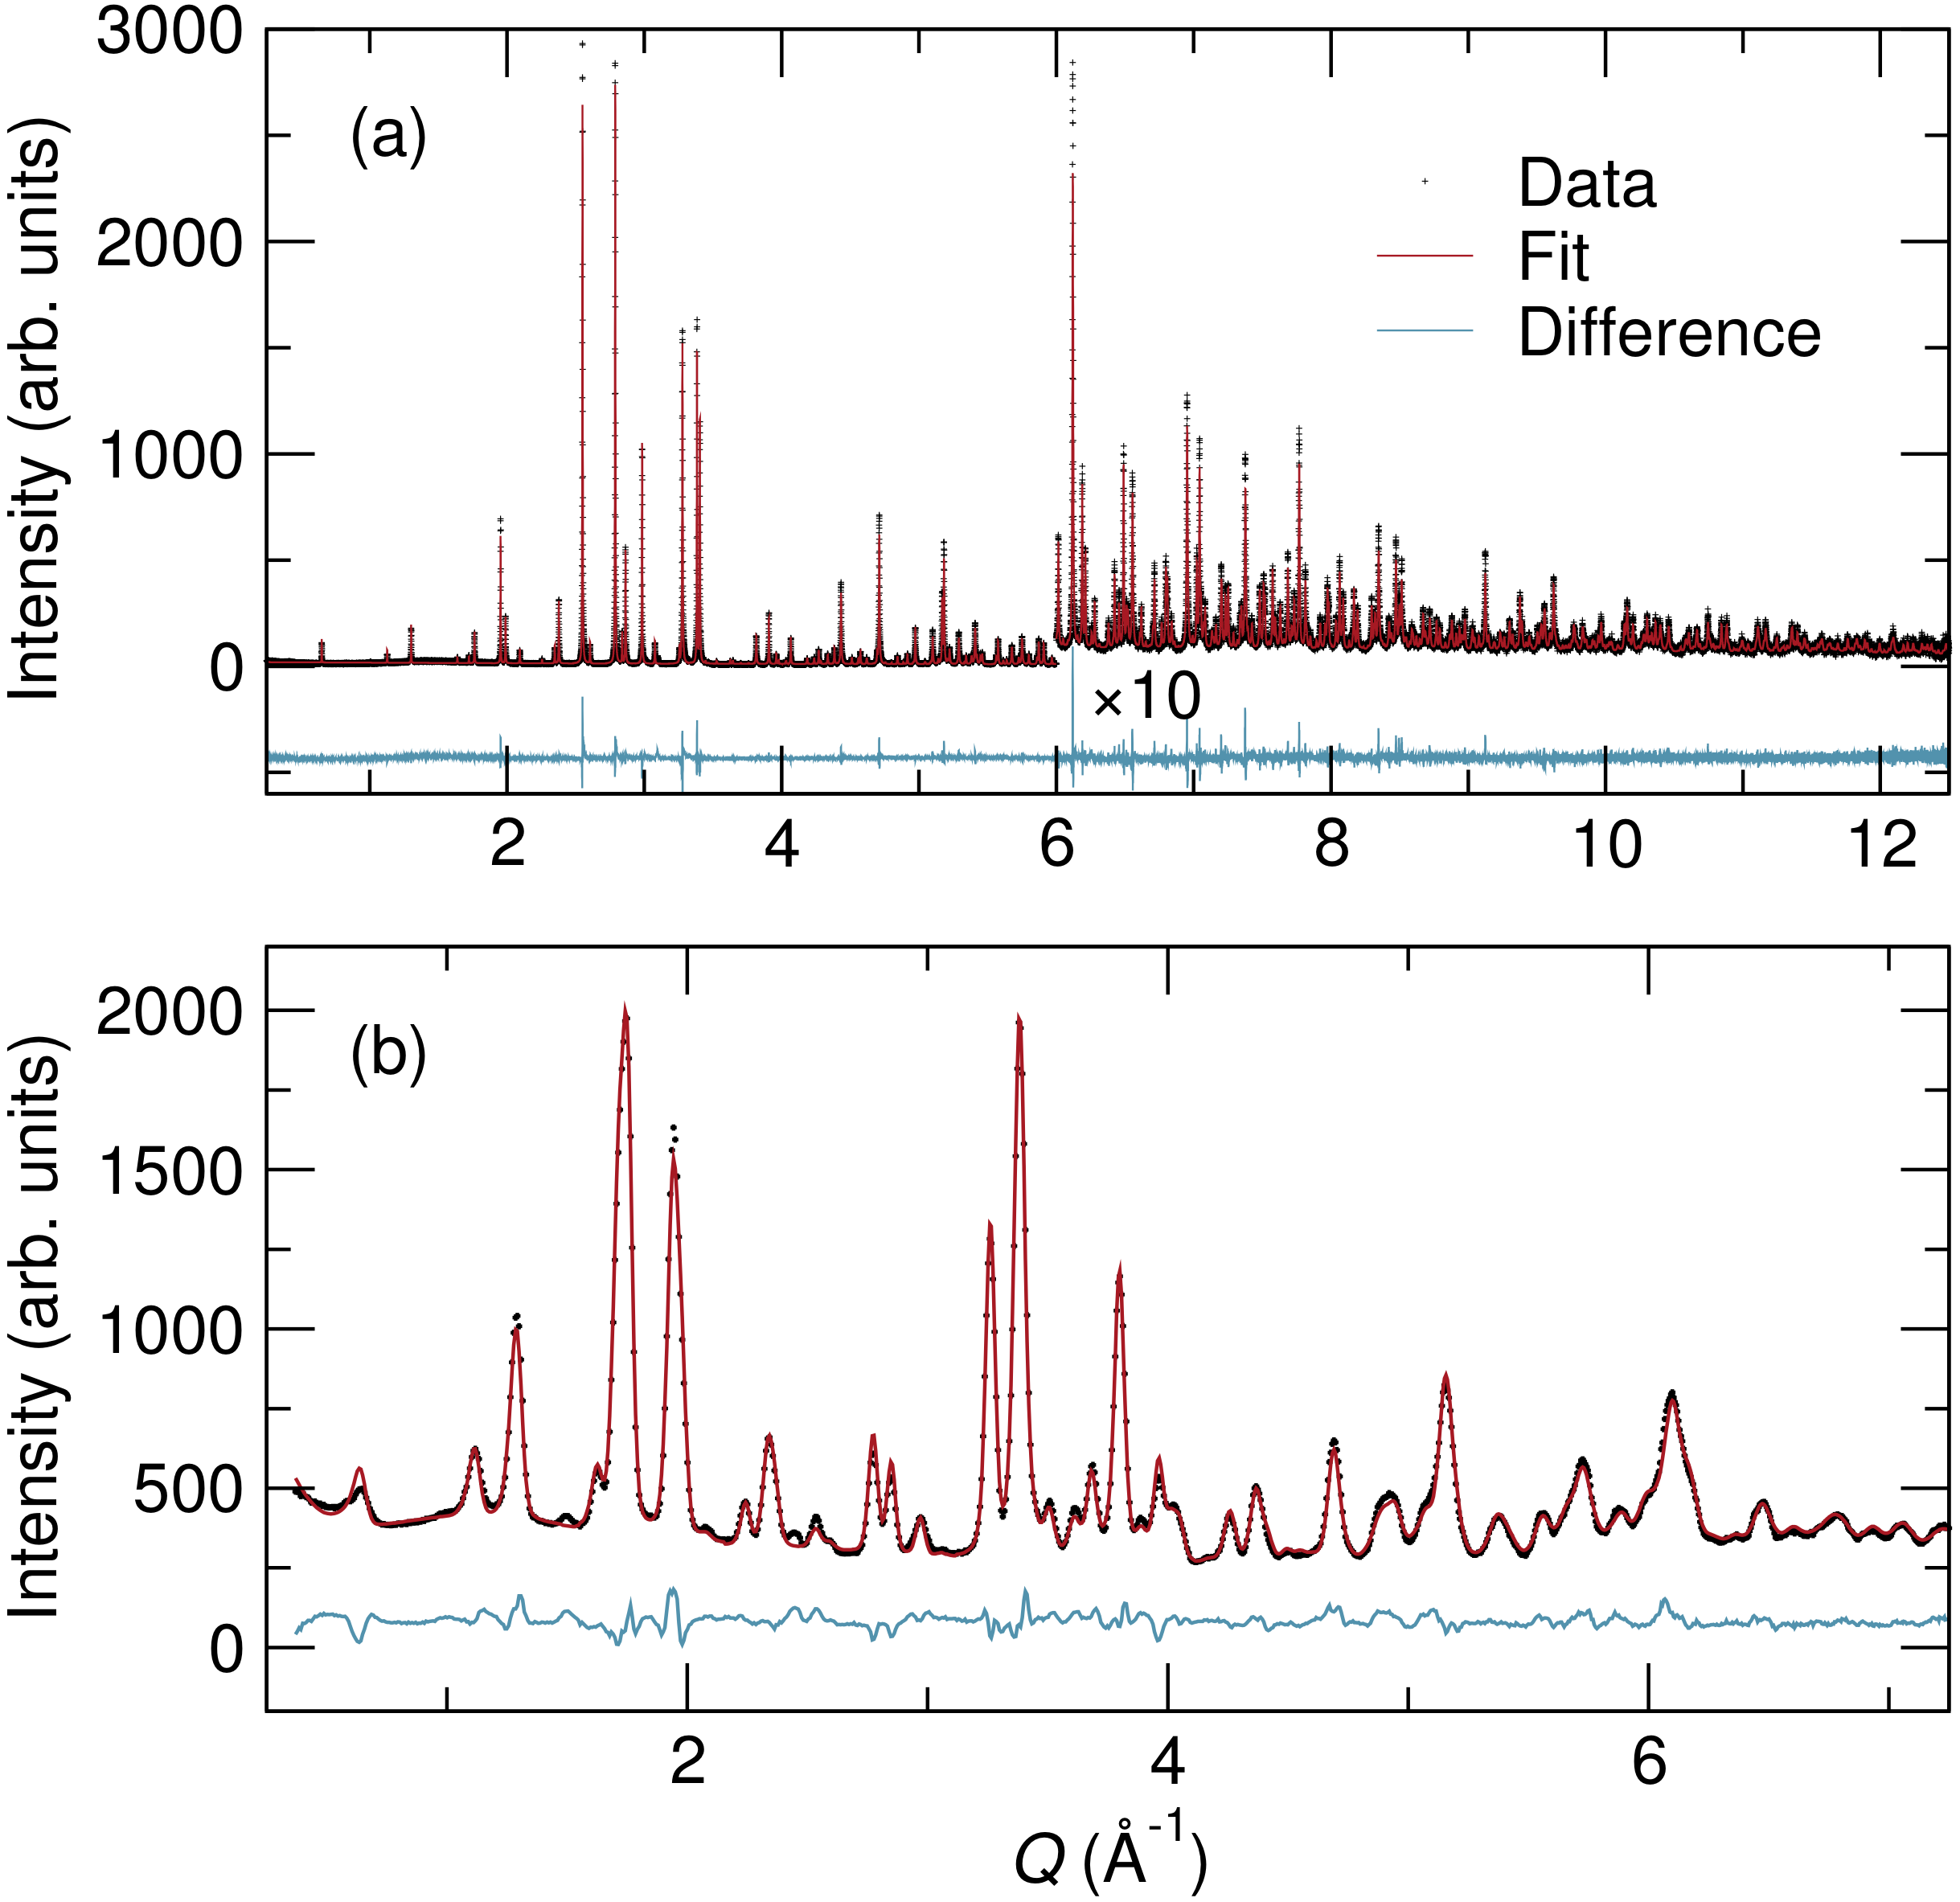
\includegraphics[width=\columnwidth]{figures/ch5/h-cumnas_11bm_100k_wand_400k_combine.png} \\
\caption{\label{fig:11BM_WAND}
Electronic band structure
}
\end{figure}

\begin{figure}
\centering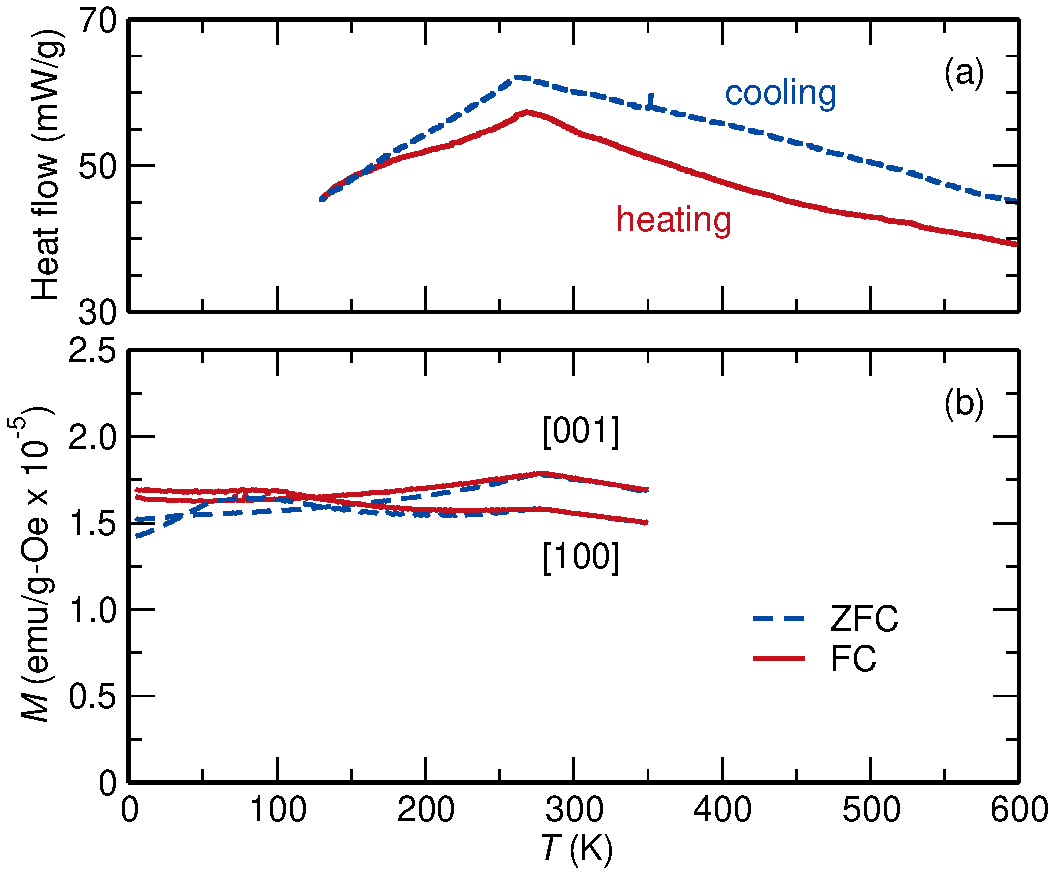
\includegraphics[width=\columnwidth]{figures/ch5/dsc-mpms_norm_cropped.pdf} \\
\caption{\label{fig:dsc_mpms}
Electronic band structure
}
\end{figure}

\begin{figure}
\centering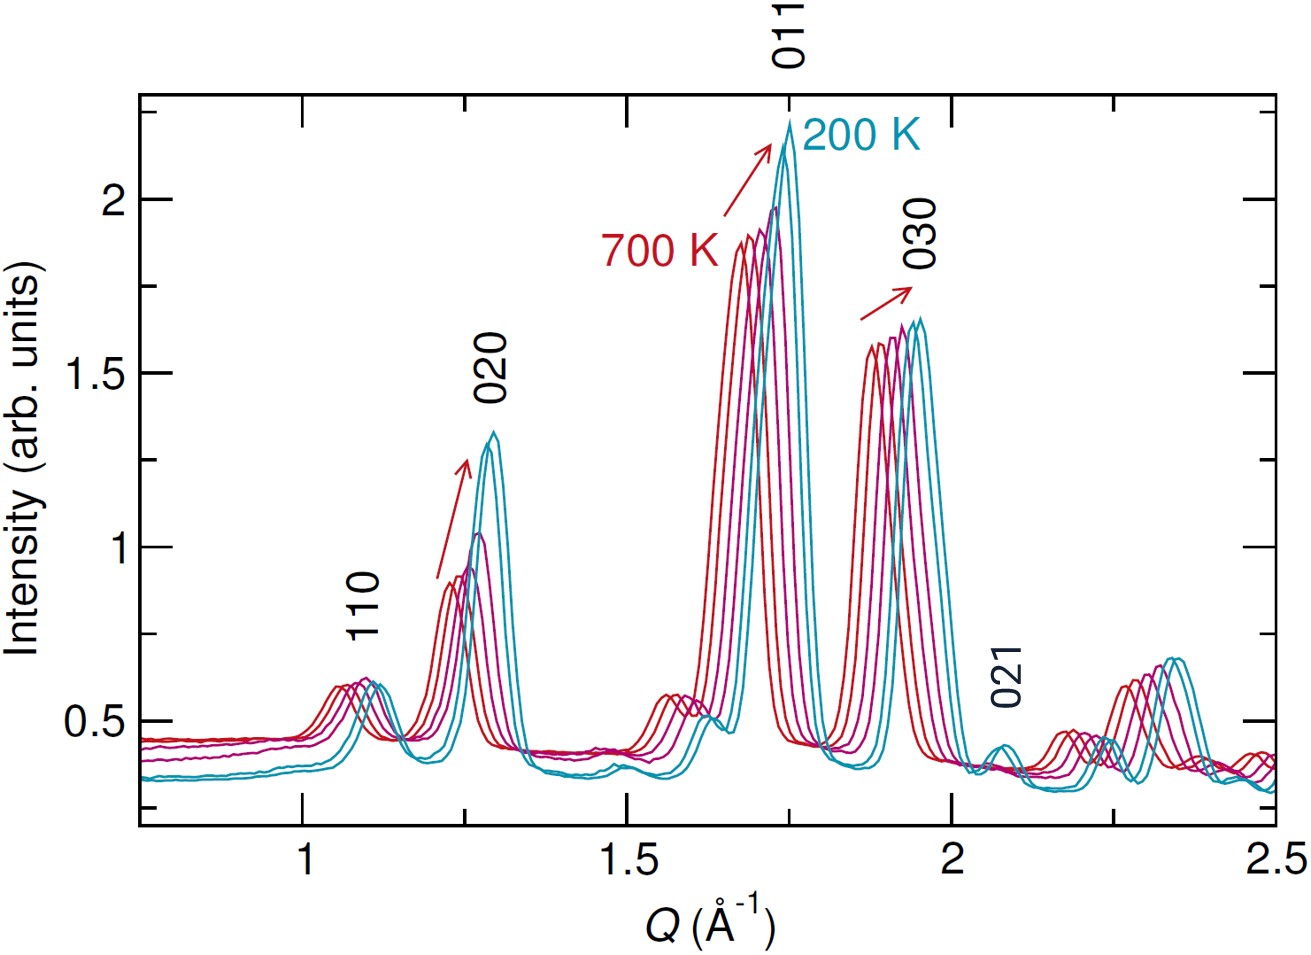
\includegraphics[width=\columnwidth]{figures/ch5/WAND_data.png} \\
\caption{\label{fig:WAND_data}
Electronic band structure
}
\end{figure}

\begin{figure}
\centering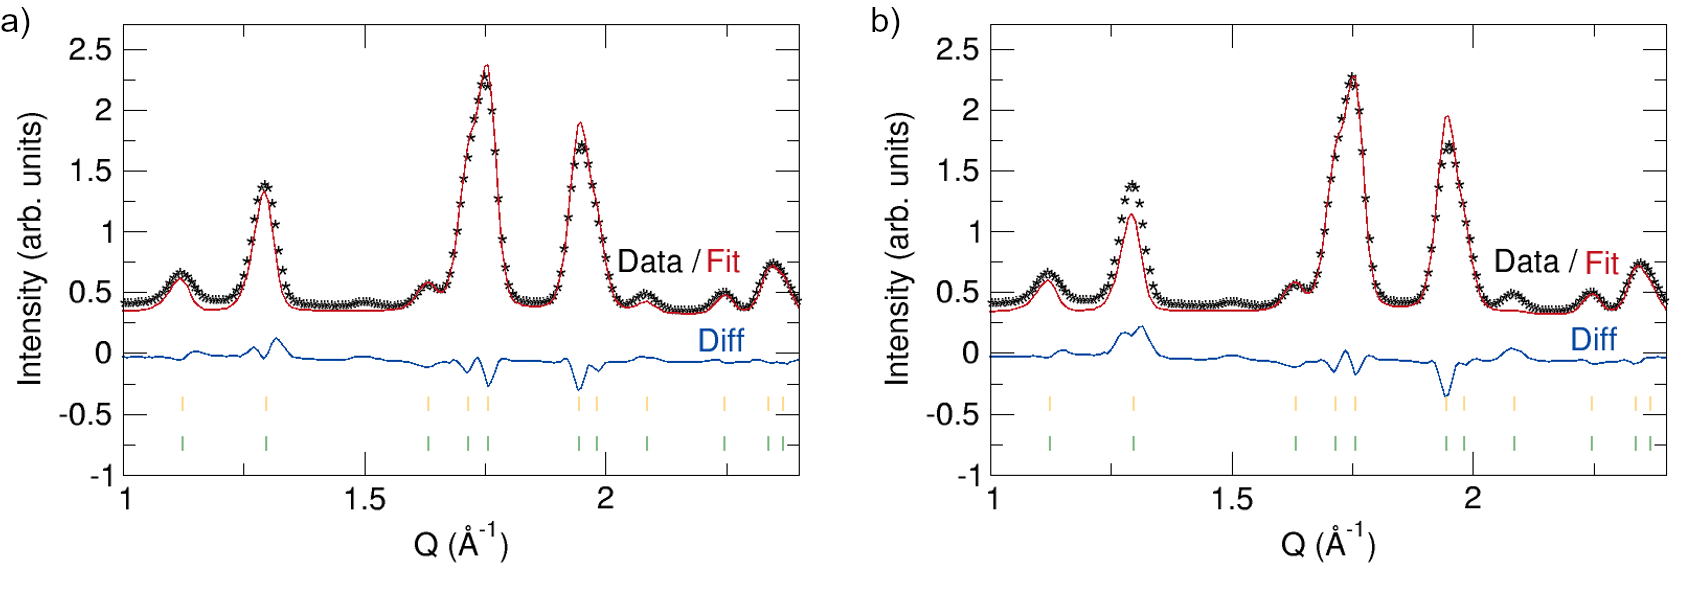
\includegraphics[width=\columnwidth]{figures/ch5/wand_refinement.png} \\
\caption{\label{fig:wand_refinement}
Electronic band structure
}
\end{figure}

\begin{figure}
\centering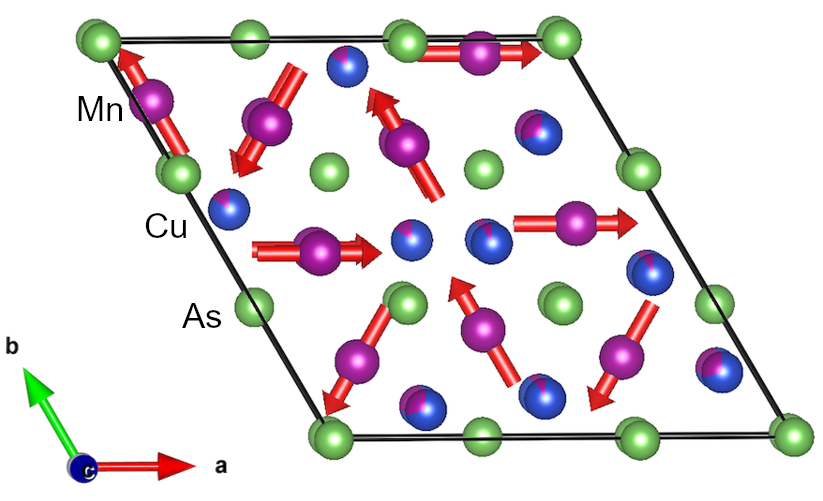
\includegraphics[width=\columnwidth]{figures/ch5/CuMnAs_magnetic_structure.png} \\
\caption{\label{fig:CuMnAs_magnetic_structure}
Electronic band structure
}
\end{figure}

\begin{figure}
\centering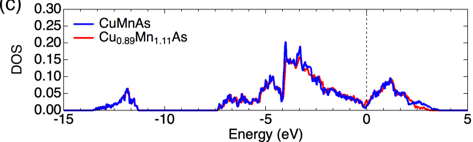
\includegraphics[width=\columnwidth]{figures/ch5/DOS_CuMnAs.png} \\
\caption{\label{fig:DOS}
Electronic band structure
}
\end{figure}

\begin{figure}
\centering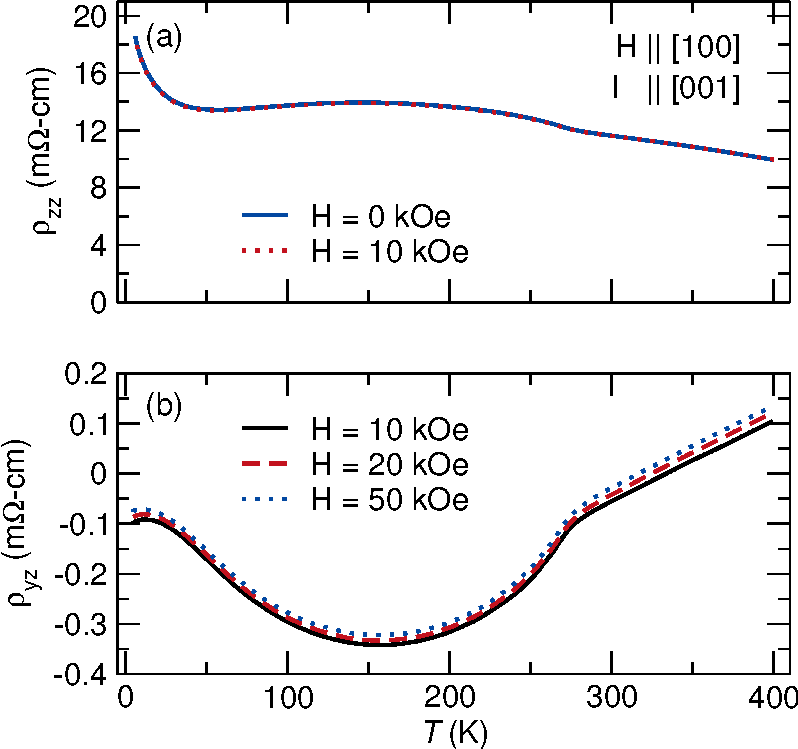
\includegraphics[width=\columnwidth]{figures/ch5/resistivity_data_hall_cropped.pdf} \\
\caption{\label{fig:resistivity}
Electronic band structure
}
\end{figure}

\Blindtext[6]

%chapter 6
\chapter{Two step magnetic ordering in monoclinic Mn$_3$As$_2$}

\begin{figure}
\centering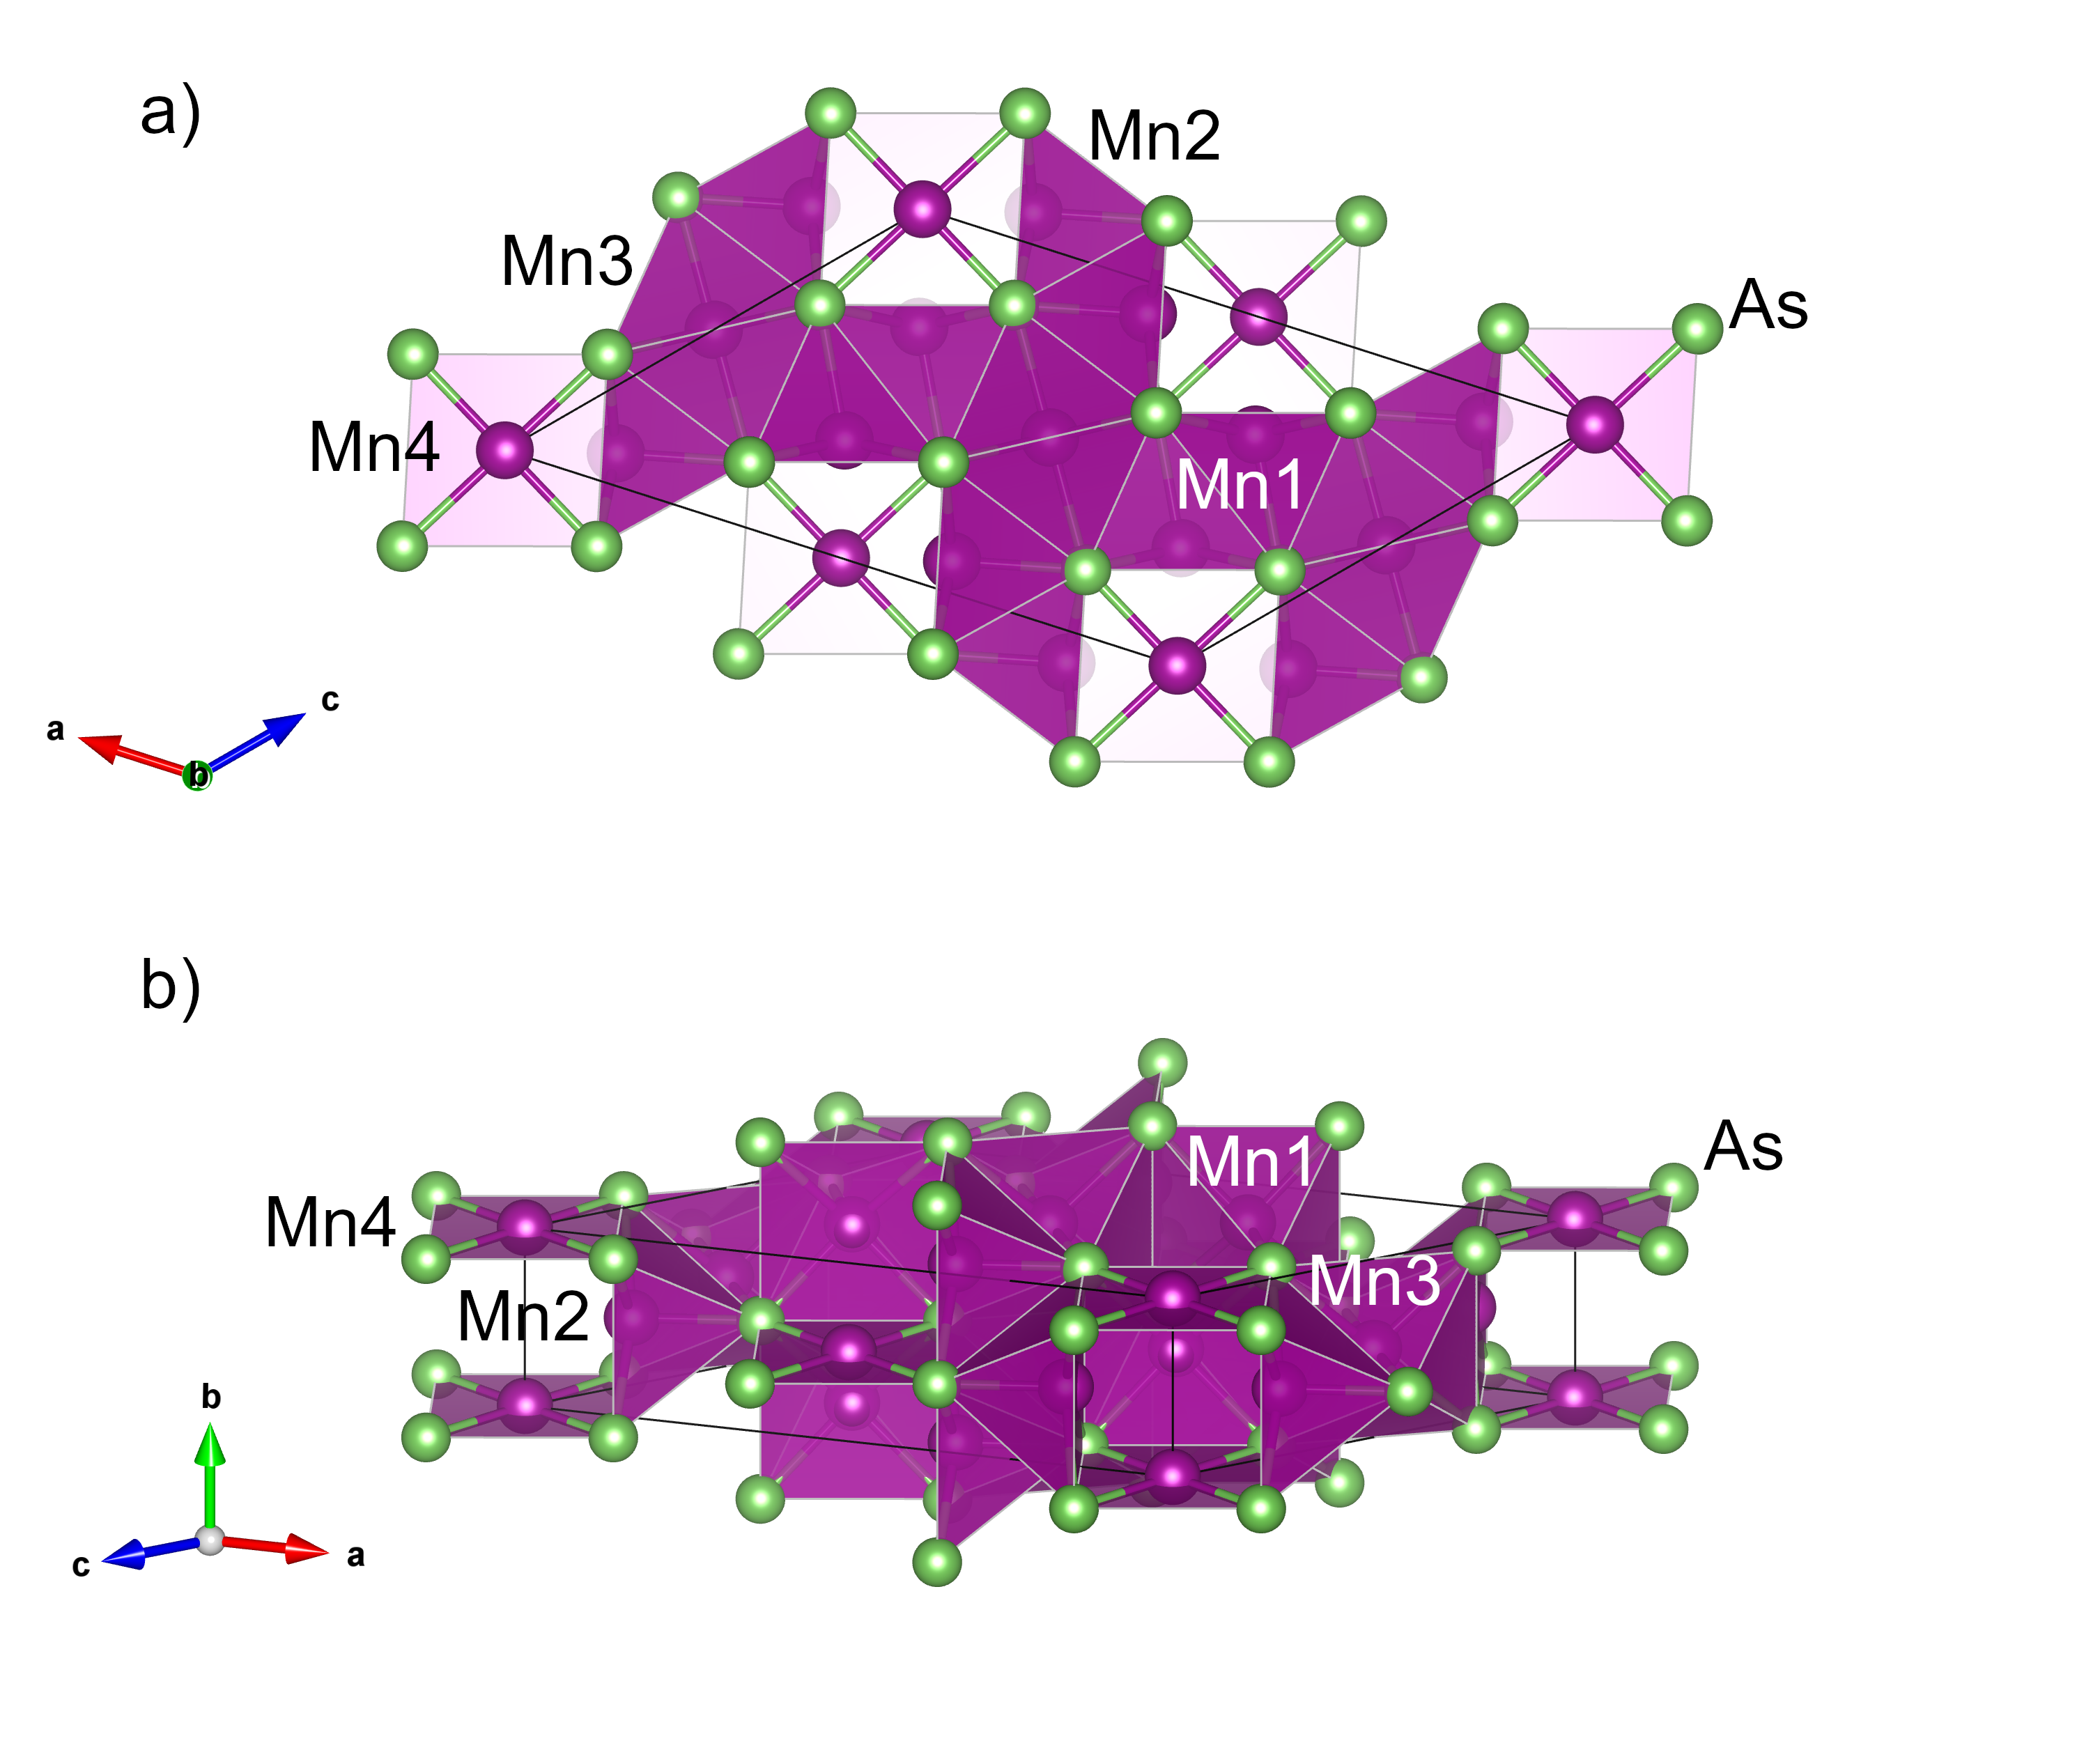
\includegraphics[width=\columnwidth]{figures/ch6/monoclinic_Mn3As2_75510.png} \\
\caption{\label{fig:Mn3As2}
Electronic band structure
}
\end{figure}

\begin{figure}
\centering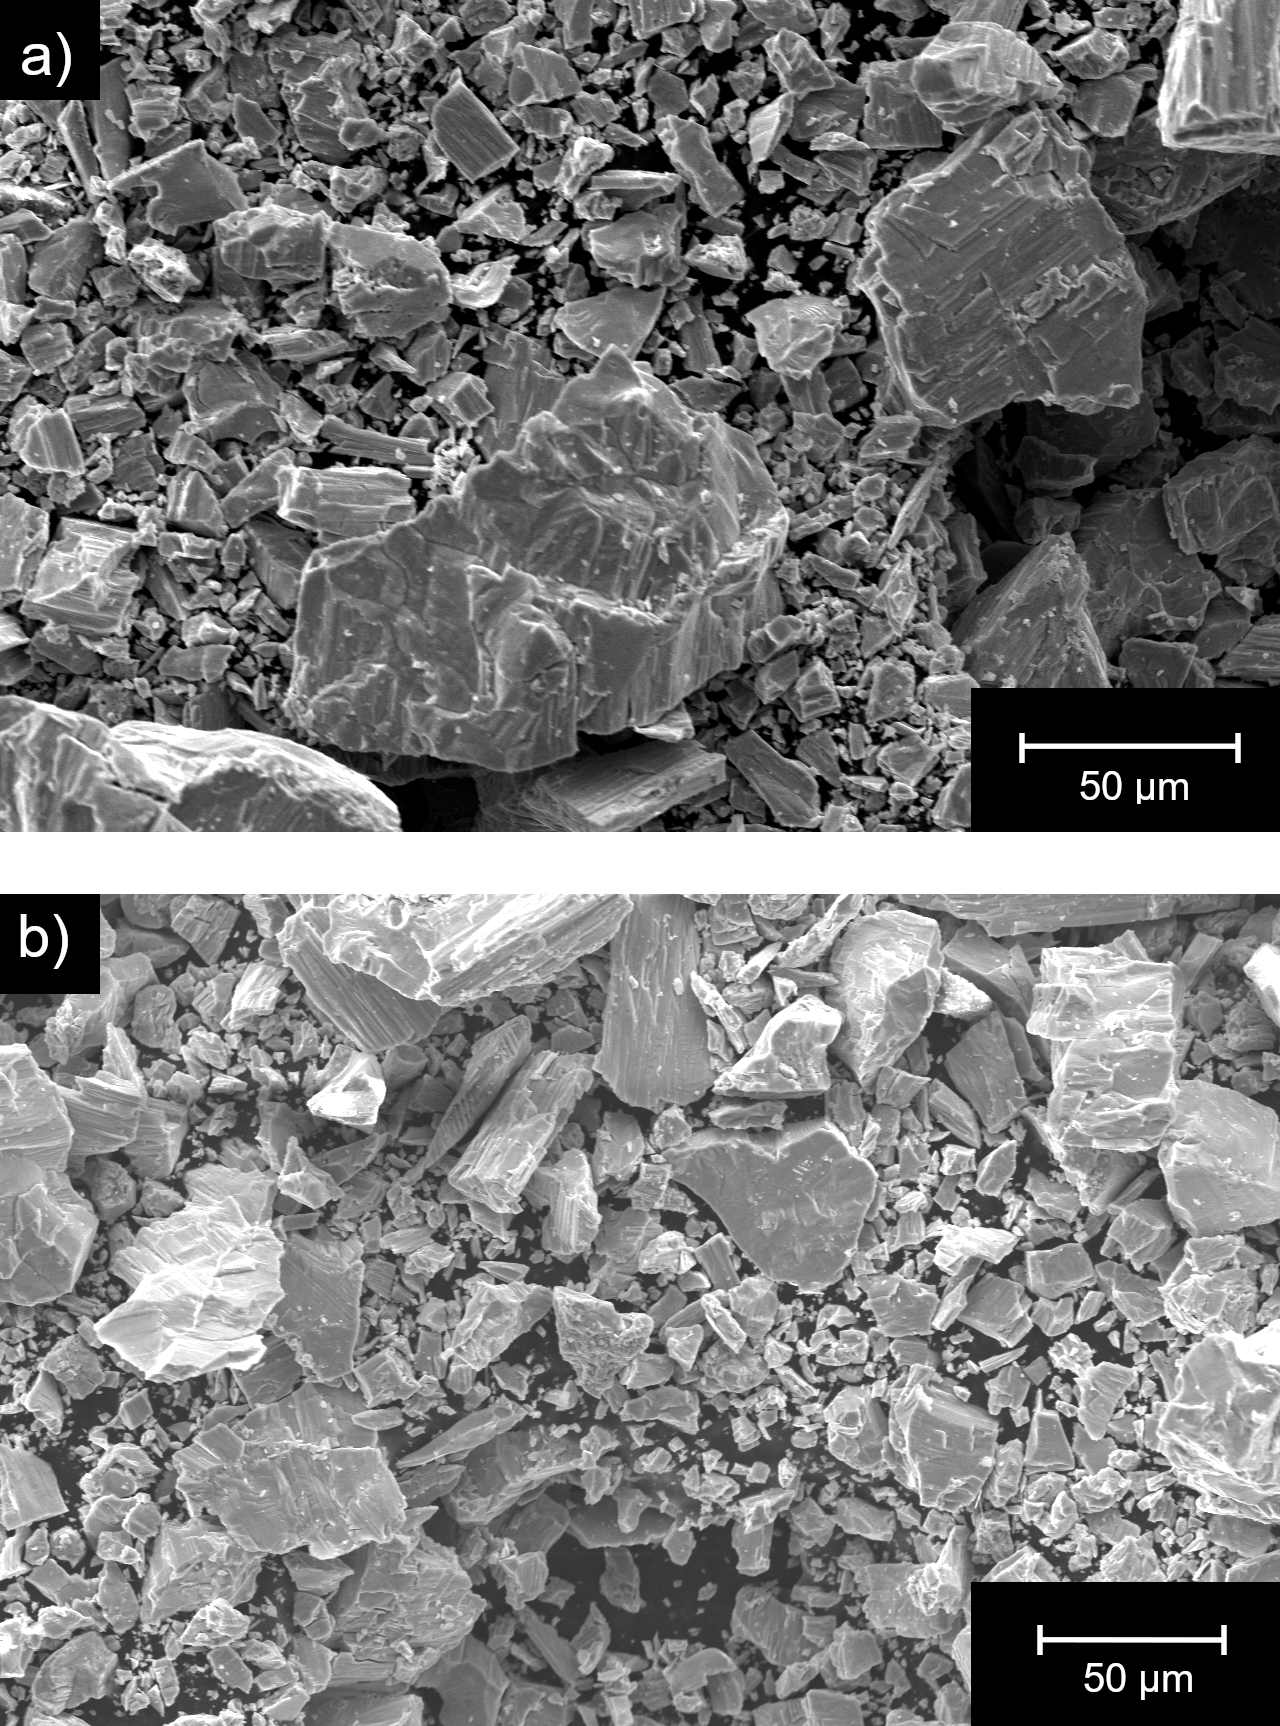
\includegraphics[width=0.5\columnwidth]{figures/ch6/Mn3As2_SEM_image.png} \\
\caption{\label{fig:Mn3As2_SEM}
Electronic band structure
}
\end{figure}

\begin{figure}
\centering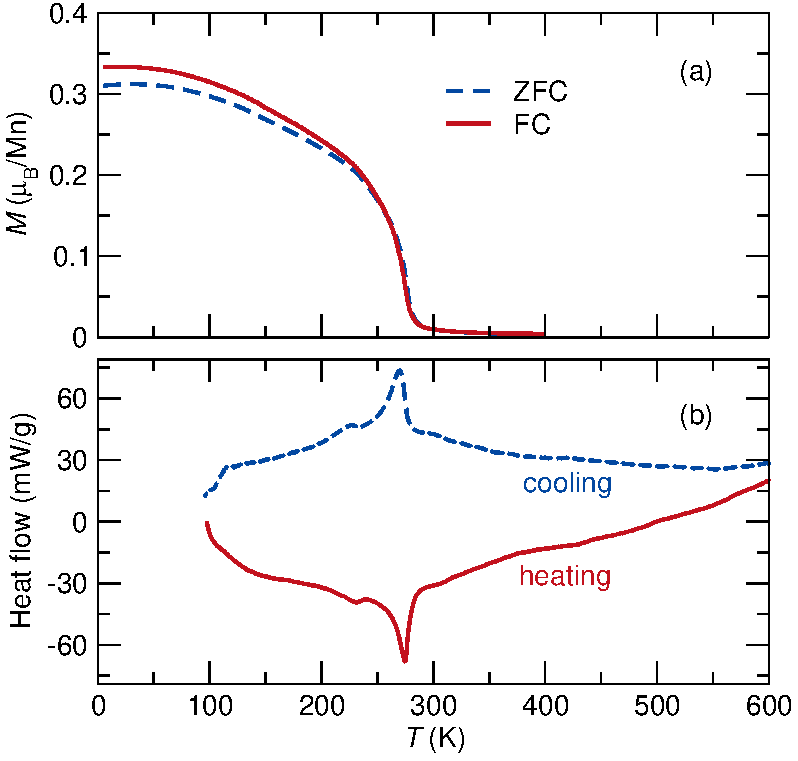
\includegraphics[width=\columnwidth]{figures/ch6/FC_ZFC_DSC_Mn3As2_cropped.pdf} \\
\caption{\label{fig:Mn3As2_FC_ZFC_DSC}
Electronic band structure
}
\end{figure}

\begin{figure}
\centering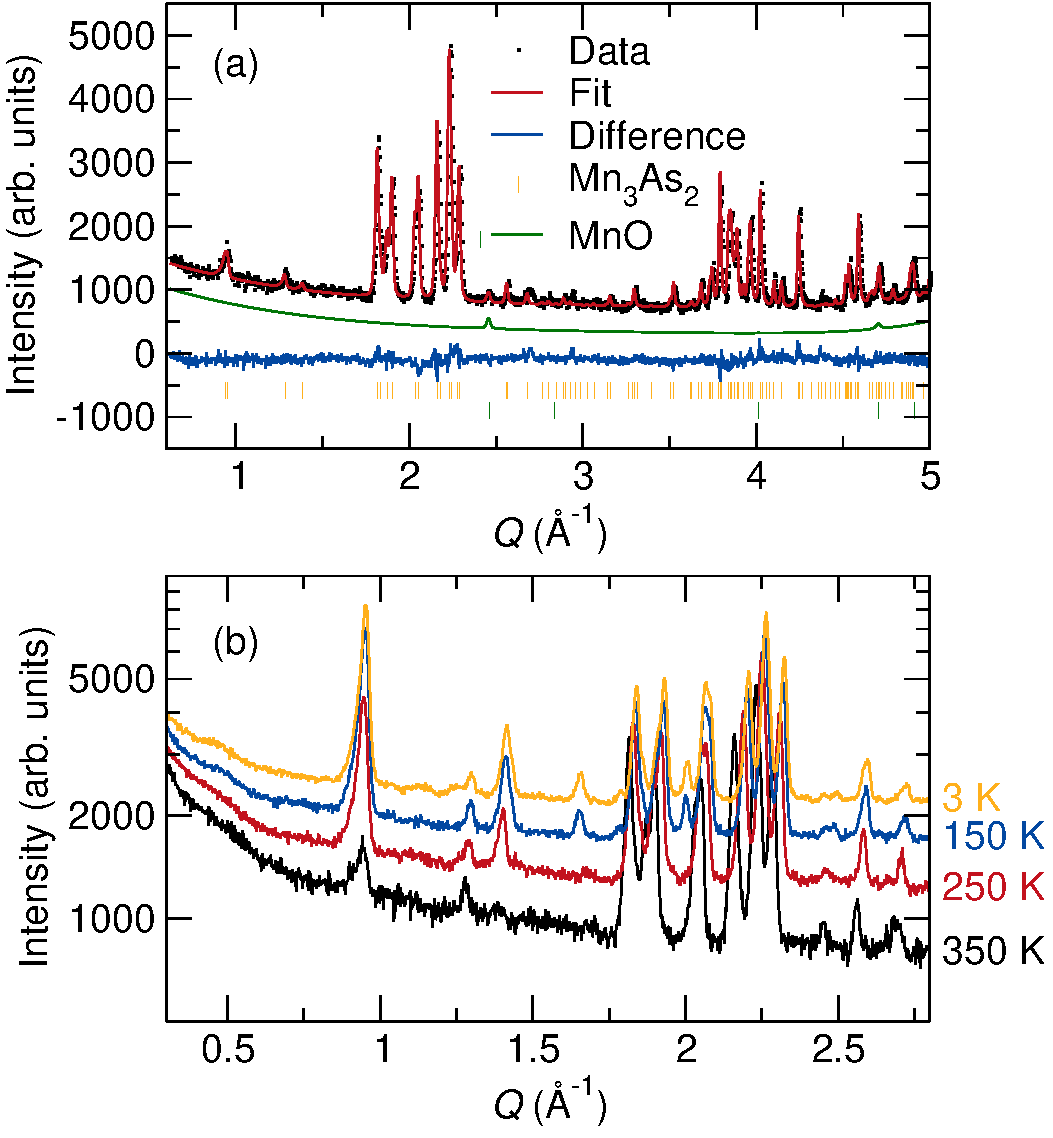
\includegraphics[width=\columnwidth]{figures/ch6/350K_rietveld_diff_temp_NPD_cropped.pdf} \\
\caption{\label{fig:350K}
Electronic band structure
}
\end{figure}

\begin{figure}
\centering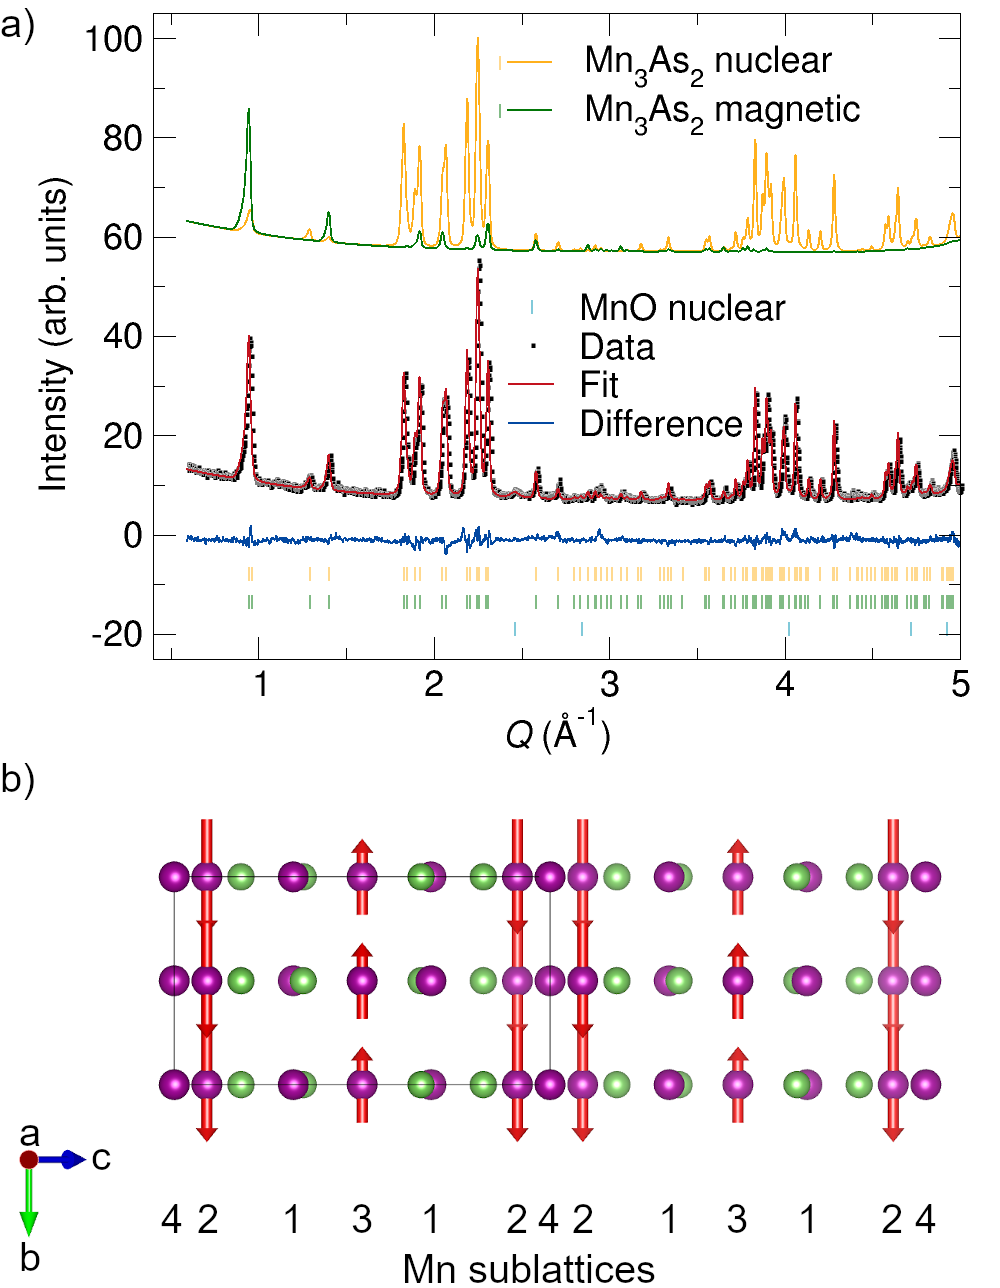
\includegraphics[width=\columnwidth]{figures/ch6/250K_mag_structure.png} \\
\caption{\label{fig:250K}
Electronic band structure
}
\end{figure}


\begin{figure}
\centering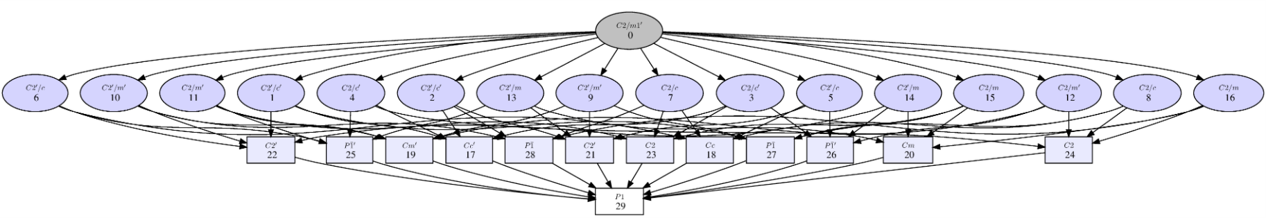
\includegraphics[width=\columnwidth]{figures/ch6/graph_of_subgraphs_3K.png} \\
\caption{\label{fig:subgraphs}
Electronic band structure
}
\end{figure}

\begin{figure}
\centering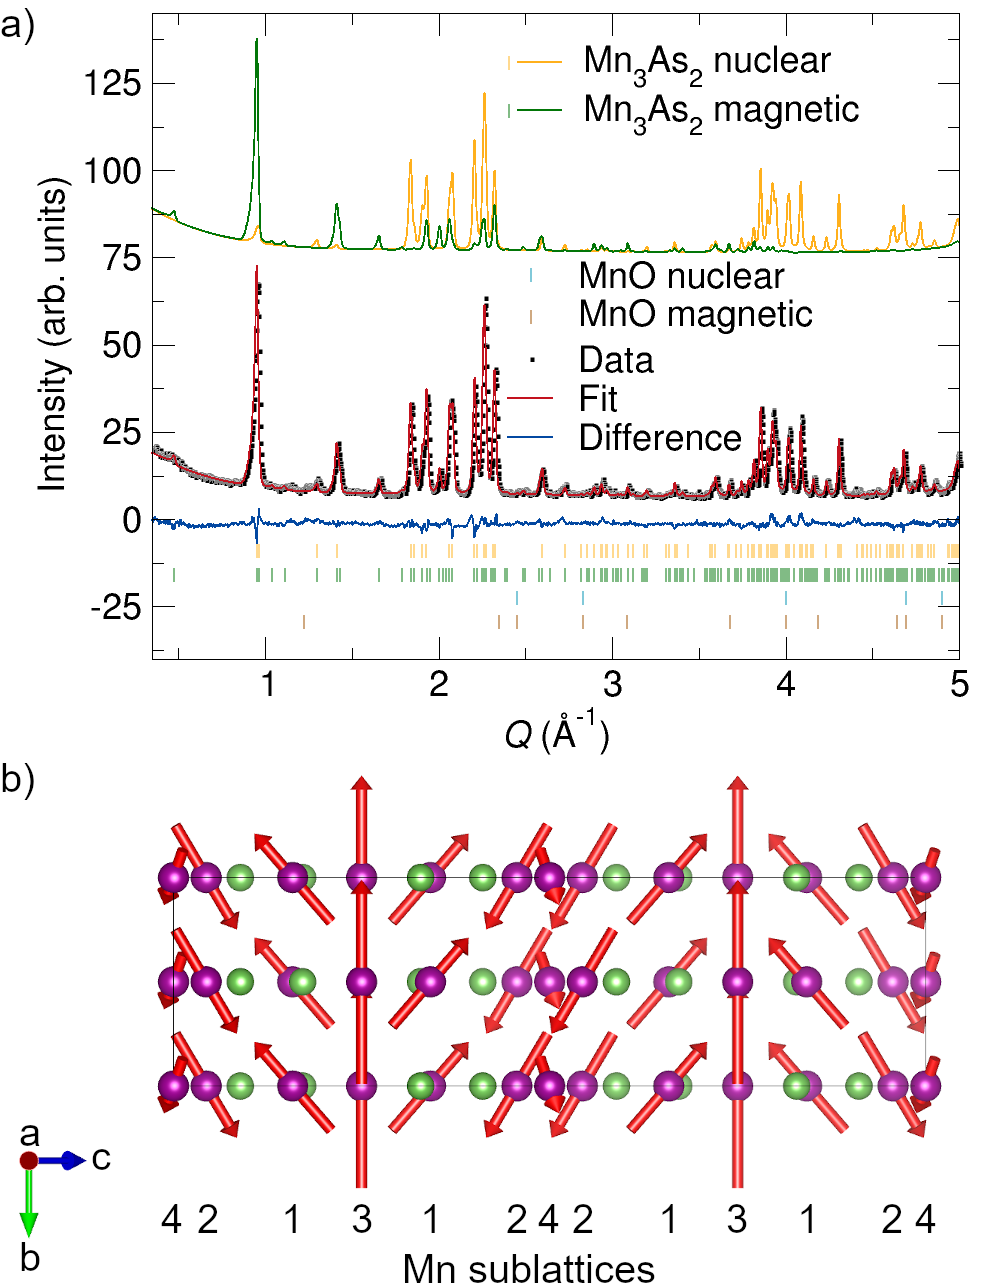
\includegraphics[width=\columnwidth]{figures/ch6/3K_mag_structure.png} \\
\caption{\label{fig:3K}
Electronic band structure
}
\end{figure}


\begin{figure}
\centering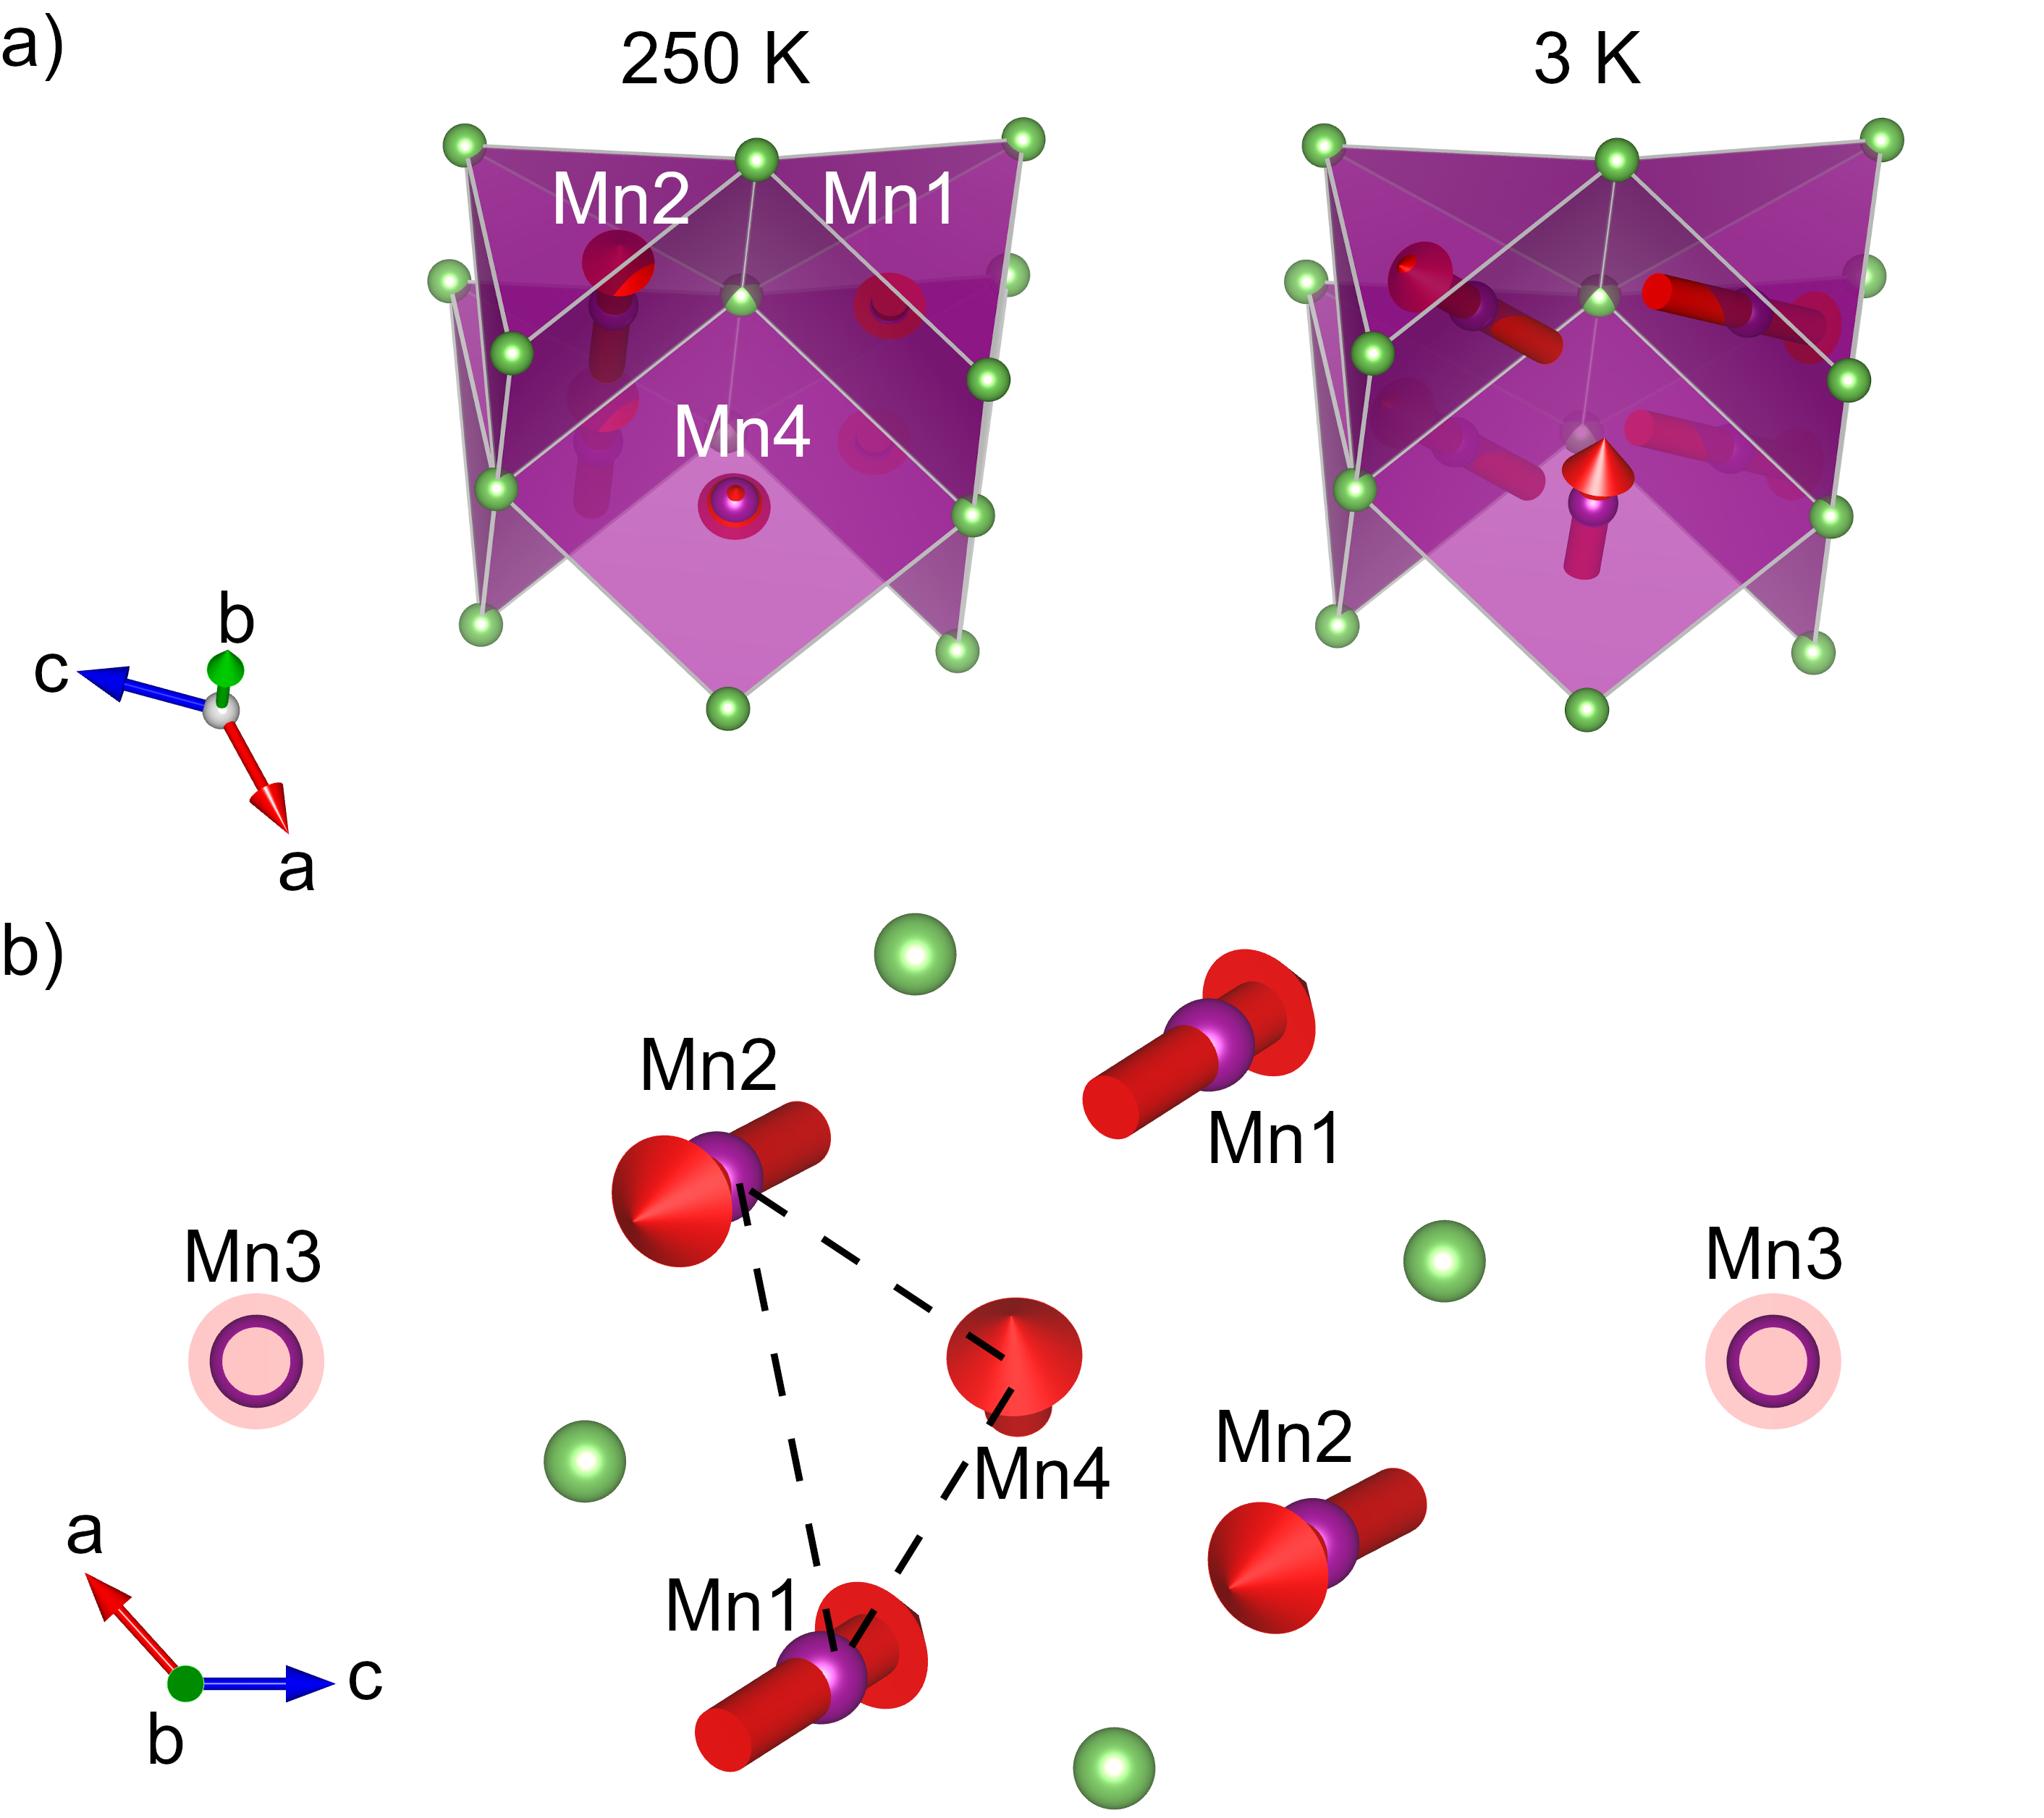
\includegraphics[width=\columnwidth]{figures/ch6/spin_canting_dps.png} \\
\caption{\label{fig:spin_canting}
Electronic band structure
}
\end{figure}

\begin{figure}
\centering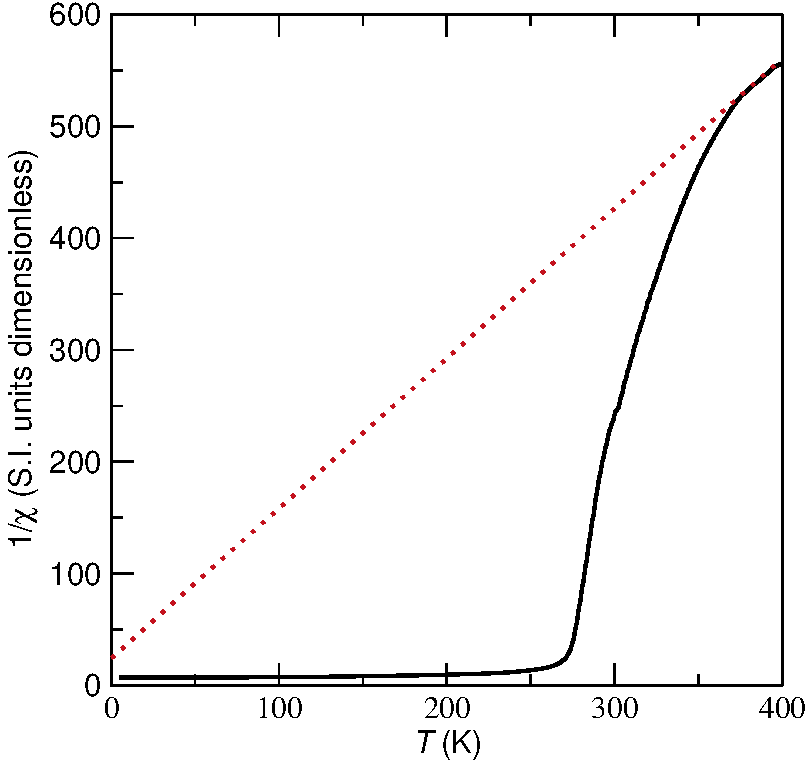
\includegraphics[width=\columnwidth]{figures/ch6/FC_52A_inverse_cropped.pdf} \\
\caption{\label{fig:inv_susceptibility}
Electronic band structure
}
\end{figure}

\Blindtext[6]

%chapter 7
\chapter{Spin canting in tetragonal CuMnAs}

\Blindtext[6]

%chapter 8
\chapter{Exchange interactions in Fe$_2$As probed by inelastic neutron scattering}

\begin{figure}
\centering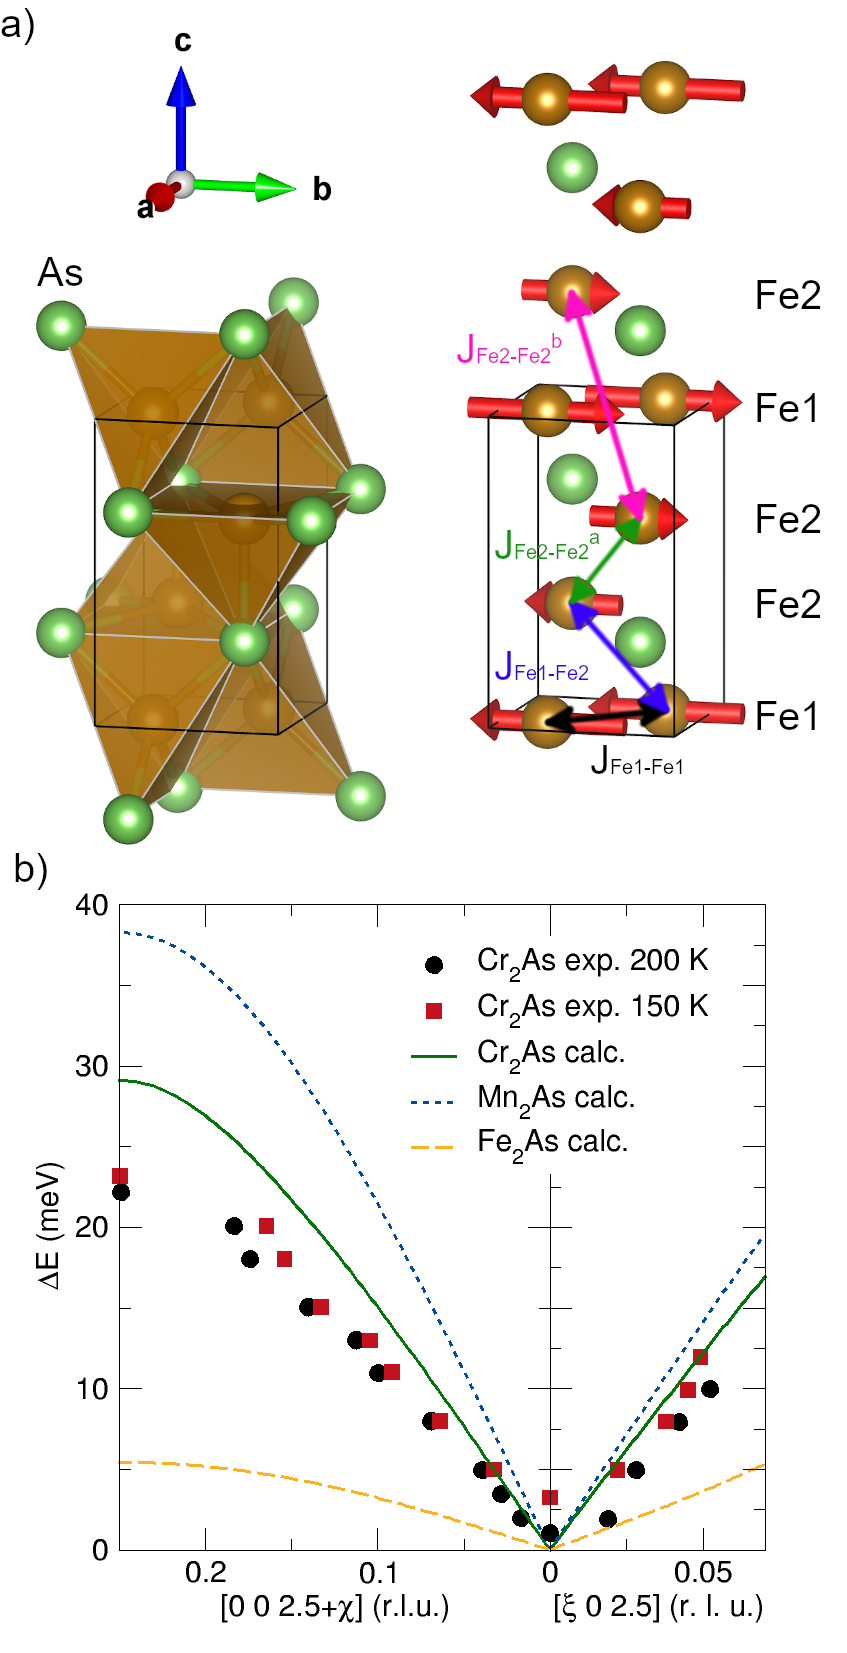
\includegraphics[width=0.5\columnwidth]{figures/ch8/Cr2As_INS_magnetic_structure.png} \\
\caption{\label{fig:Cr2As}
Electronic band structure
}
\end{figure}

\begin{figure}
\centering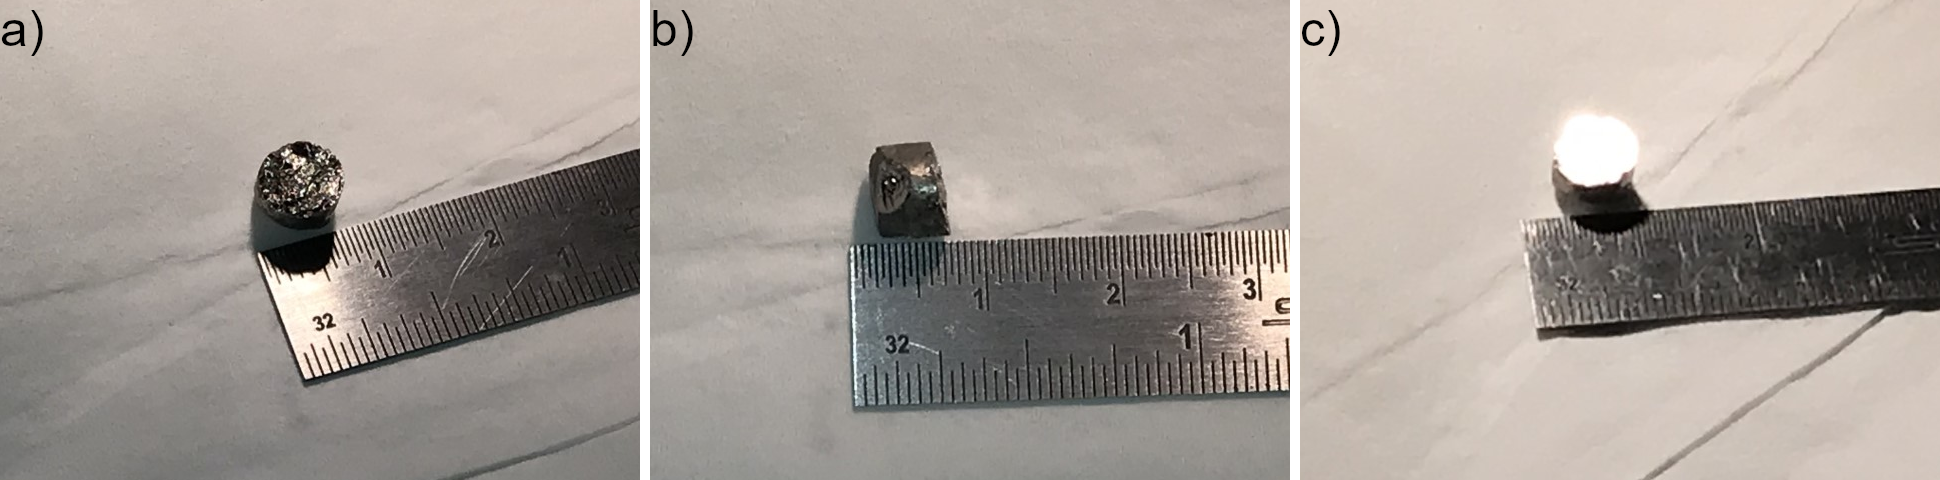
\includegraphics[width=\columnwidth]{figures/ch8/crystal.png} \\
\caption{\label{fig:crystal}
Electronic band structure
}
\end{figure}

\begin{figure}
\centering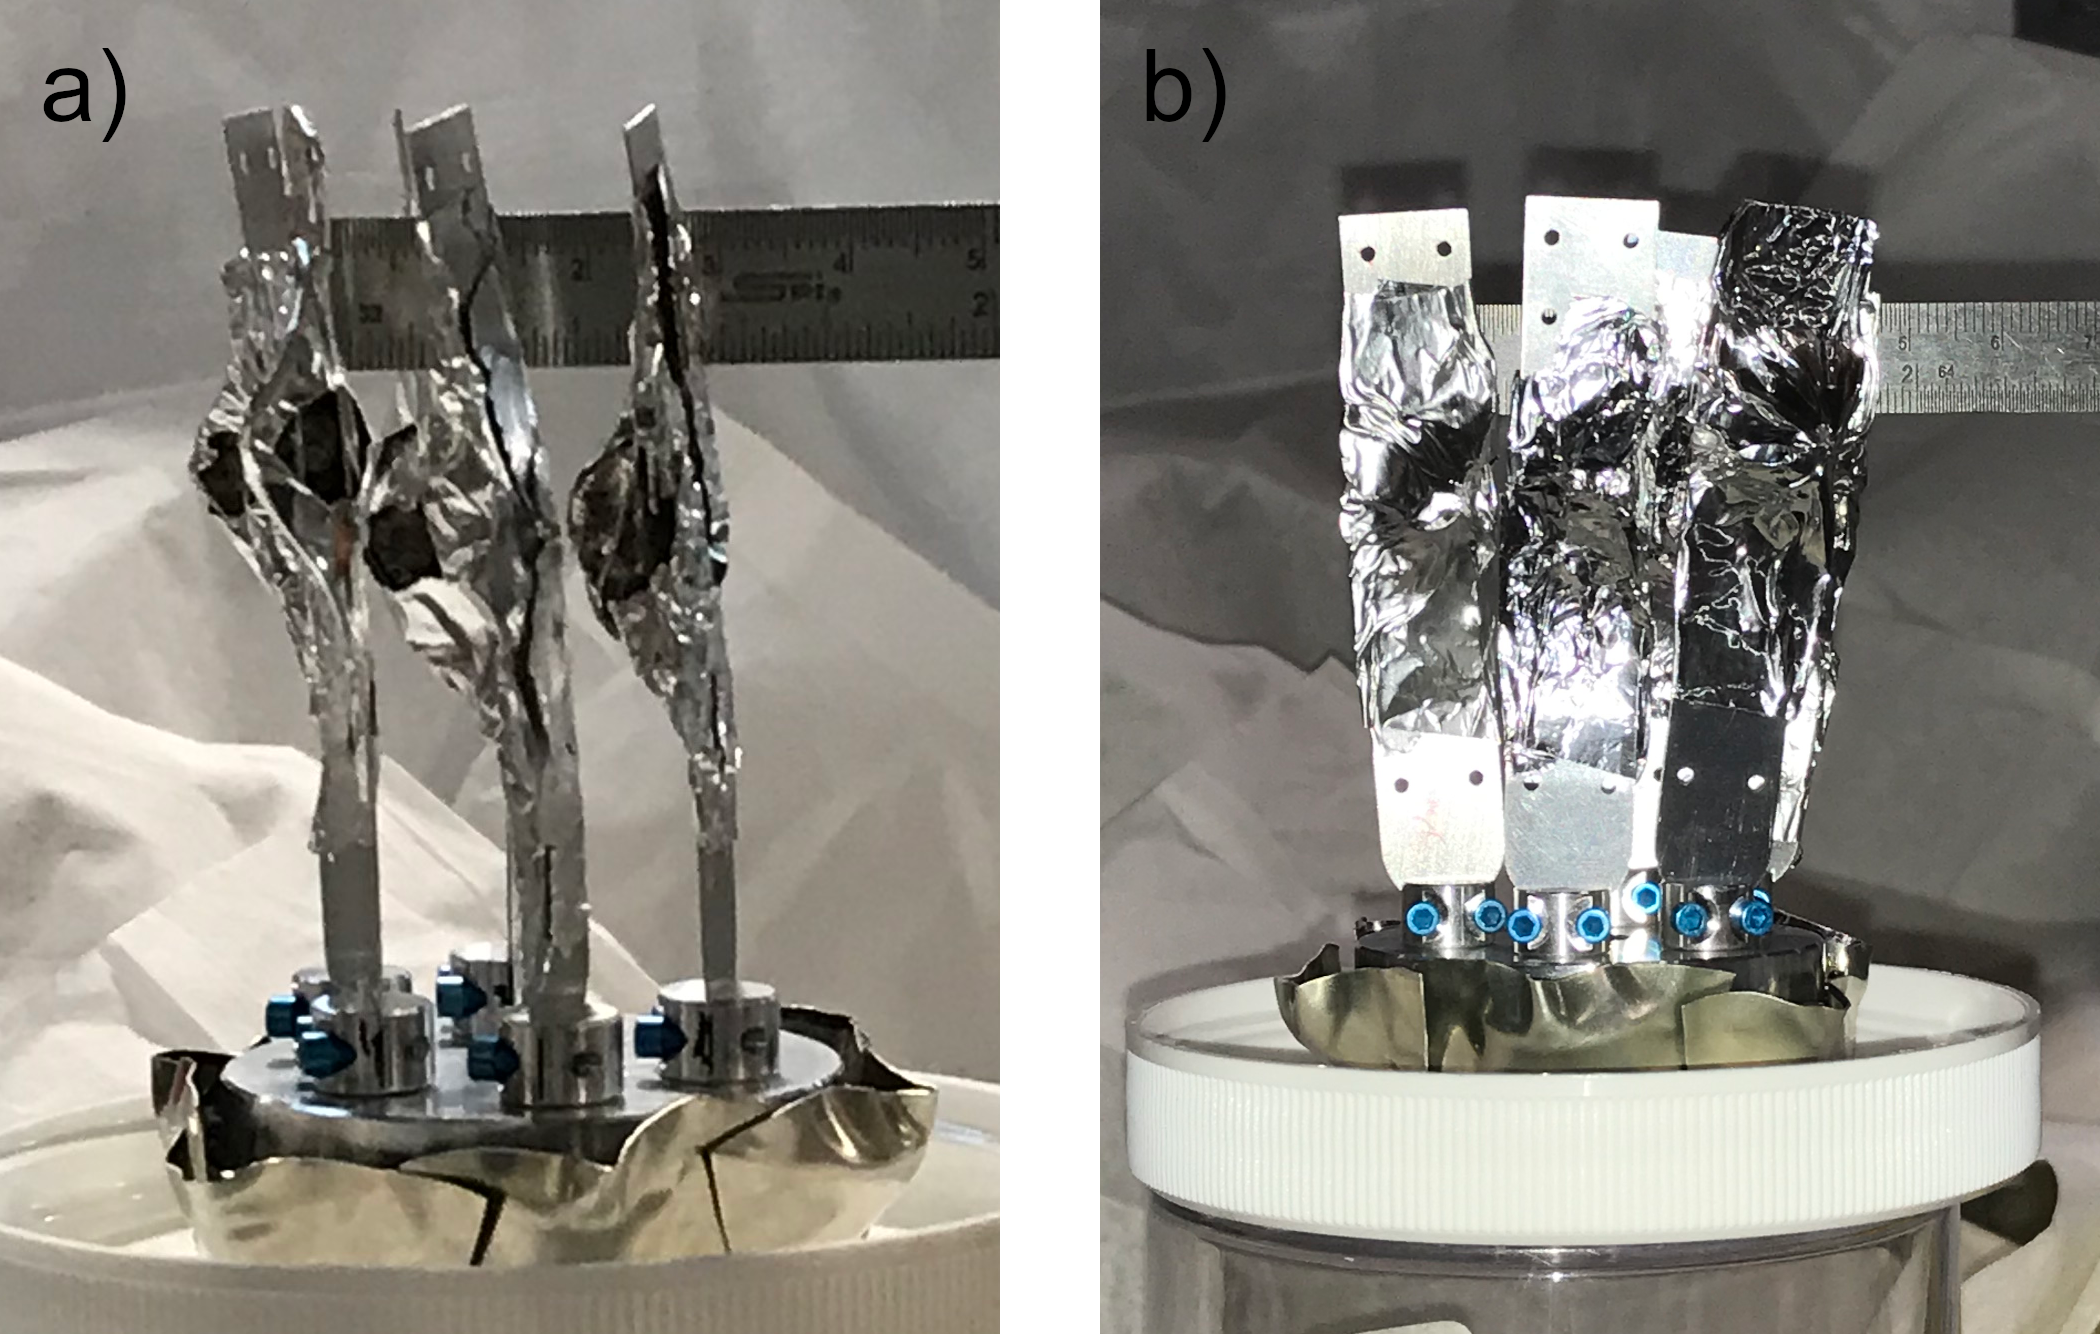
\includegraphics[width=\columnwidth]{figures/ch8/crystal_array.png} \\
\caption{\label{fig:crystal_array}
Electronic band structure
}
\end{figure}

\begin{figure}
\centering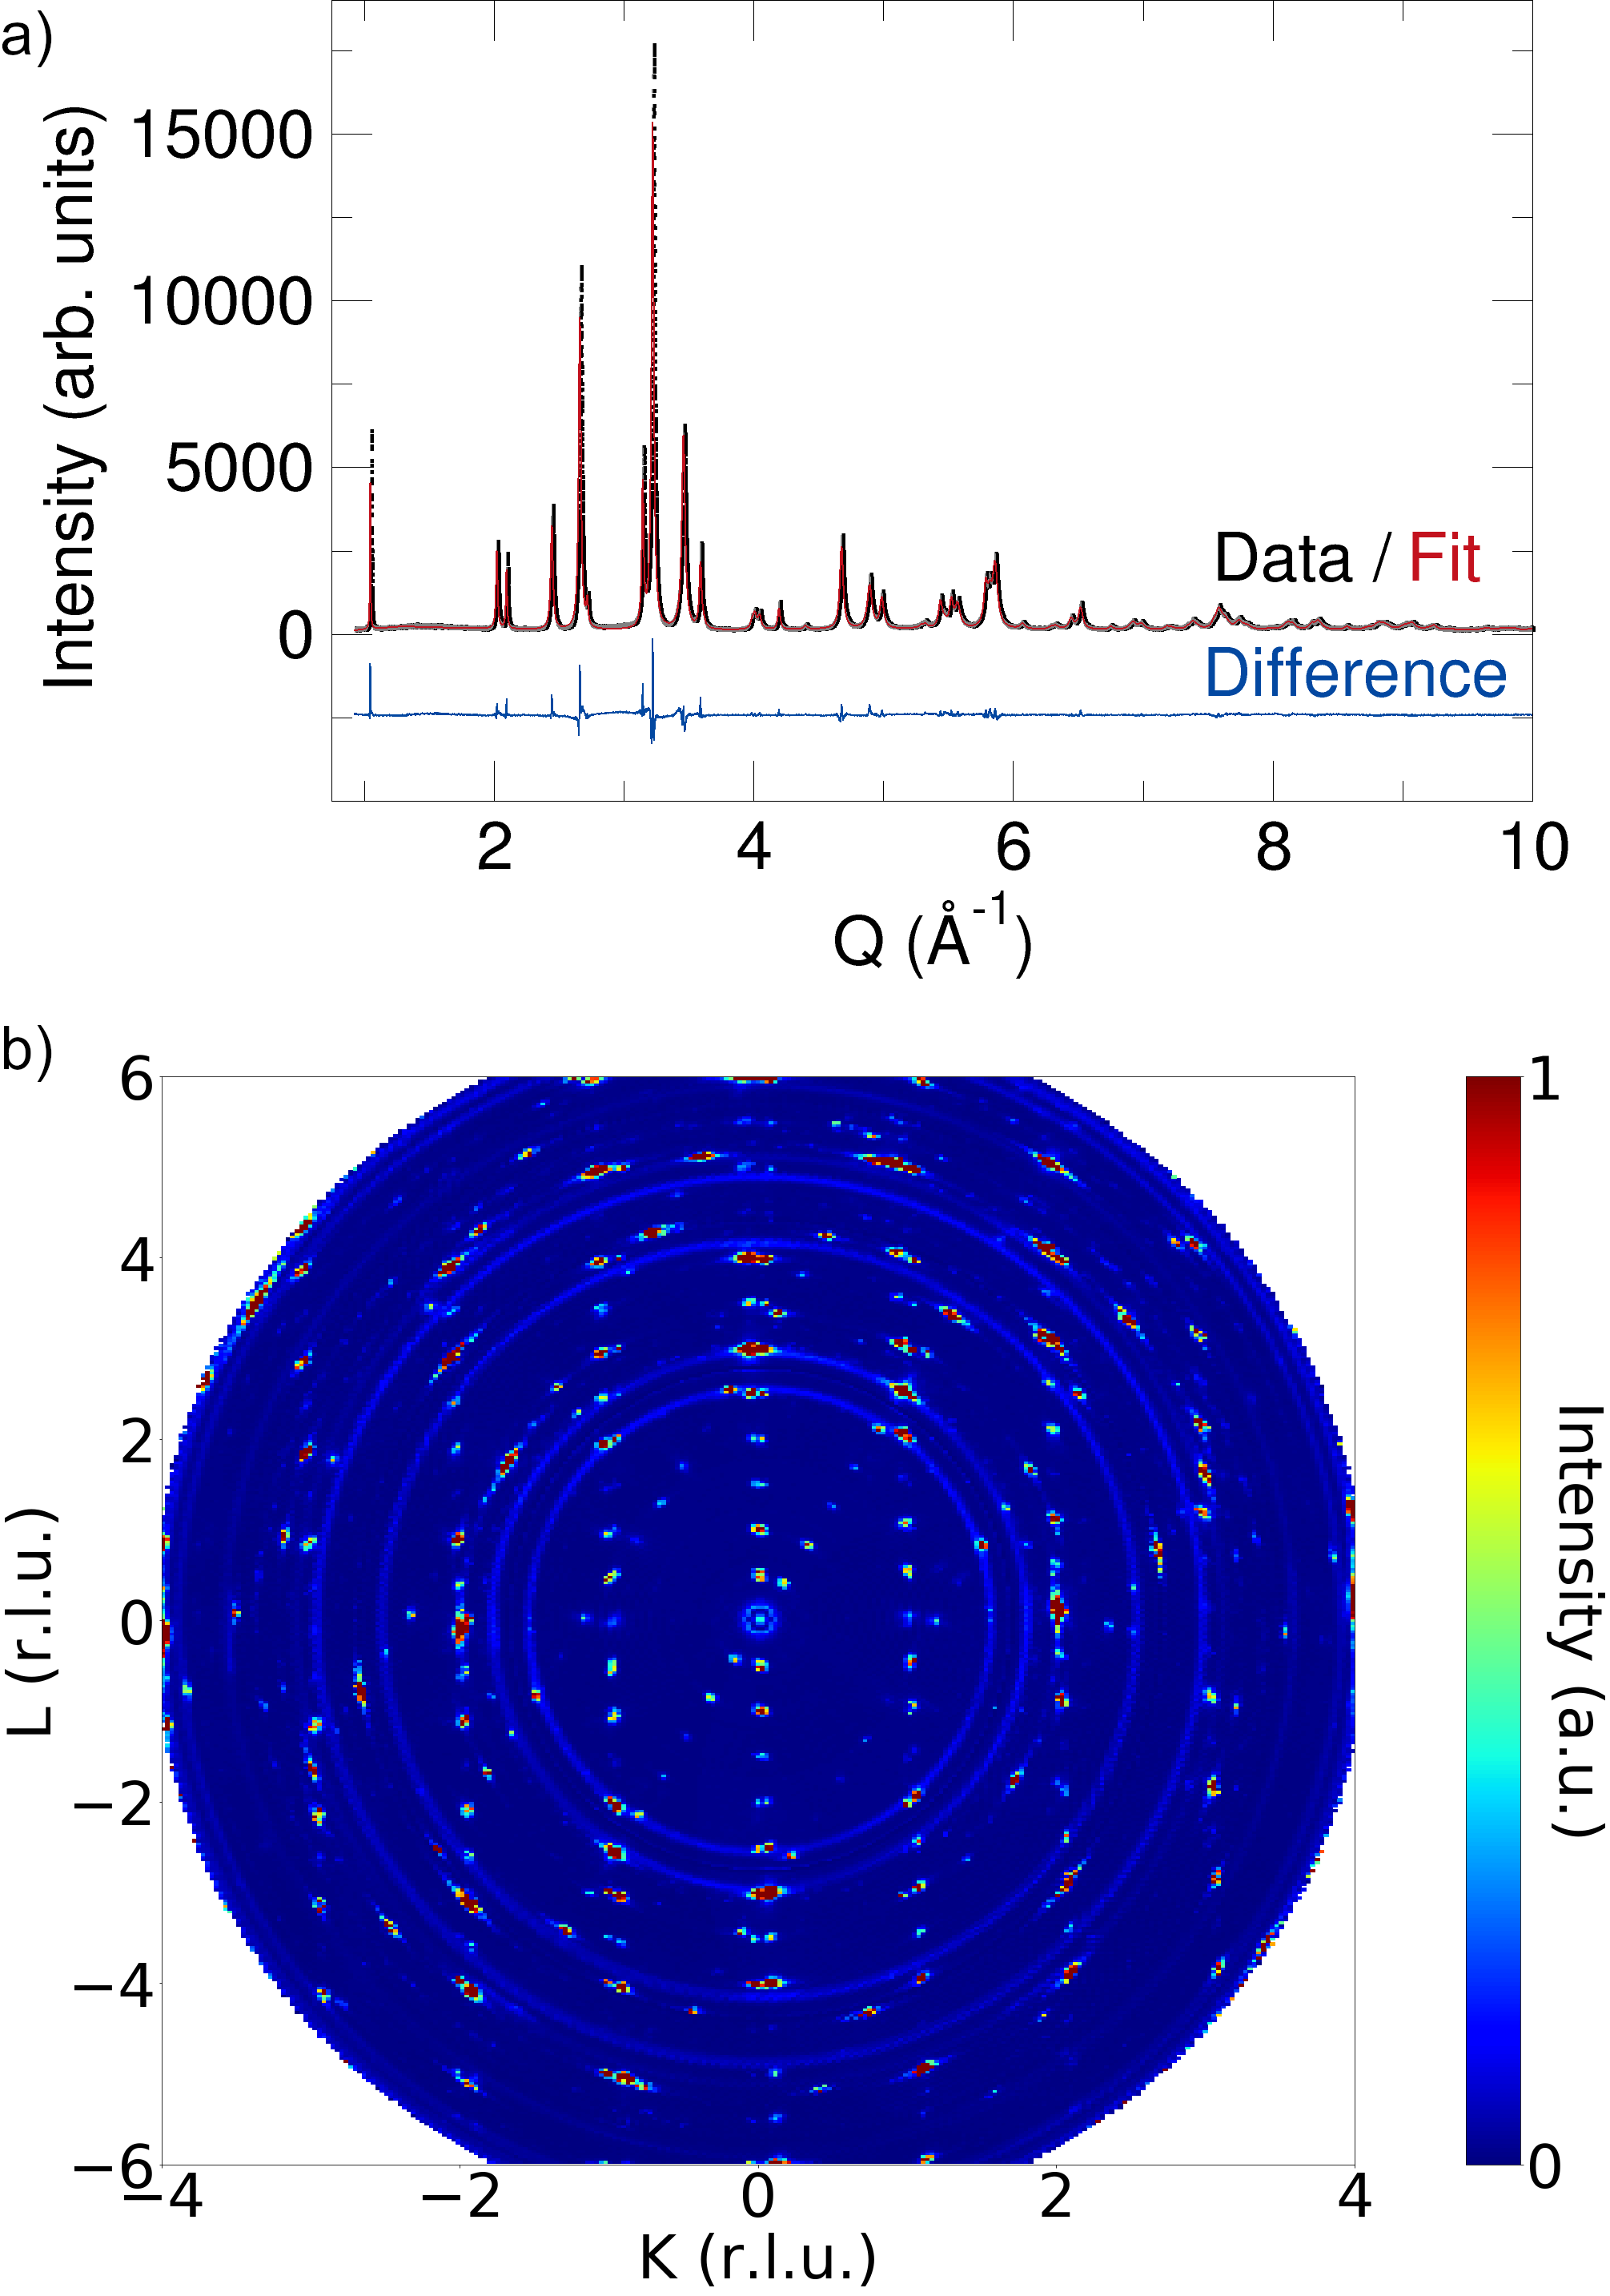
\includegraphics[width=\columnwidth]{figures/ch8/11BM_refinement_elastic_slice.png} \\
\caption{\label{fig:11BM_elastic_slice}
Electronic band structure
}
\end{figure}

\begin{figure}
\centering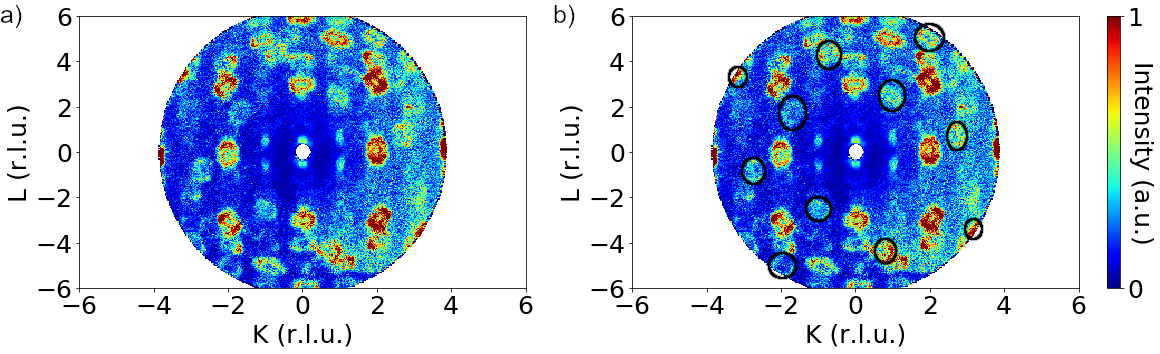
\includegraphics[width=0.7\columnwidth]{figures/ch8/suppl_misaligned_crystal_kl_slice.png} \\
\caption{\label{fig:misalign_crystal}
Electronic band structure
}
\end{figure}

\begin{figure}
\centering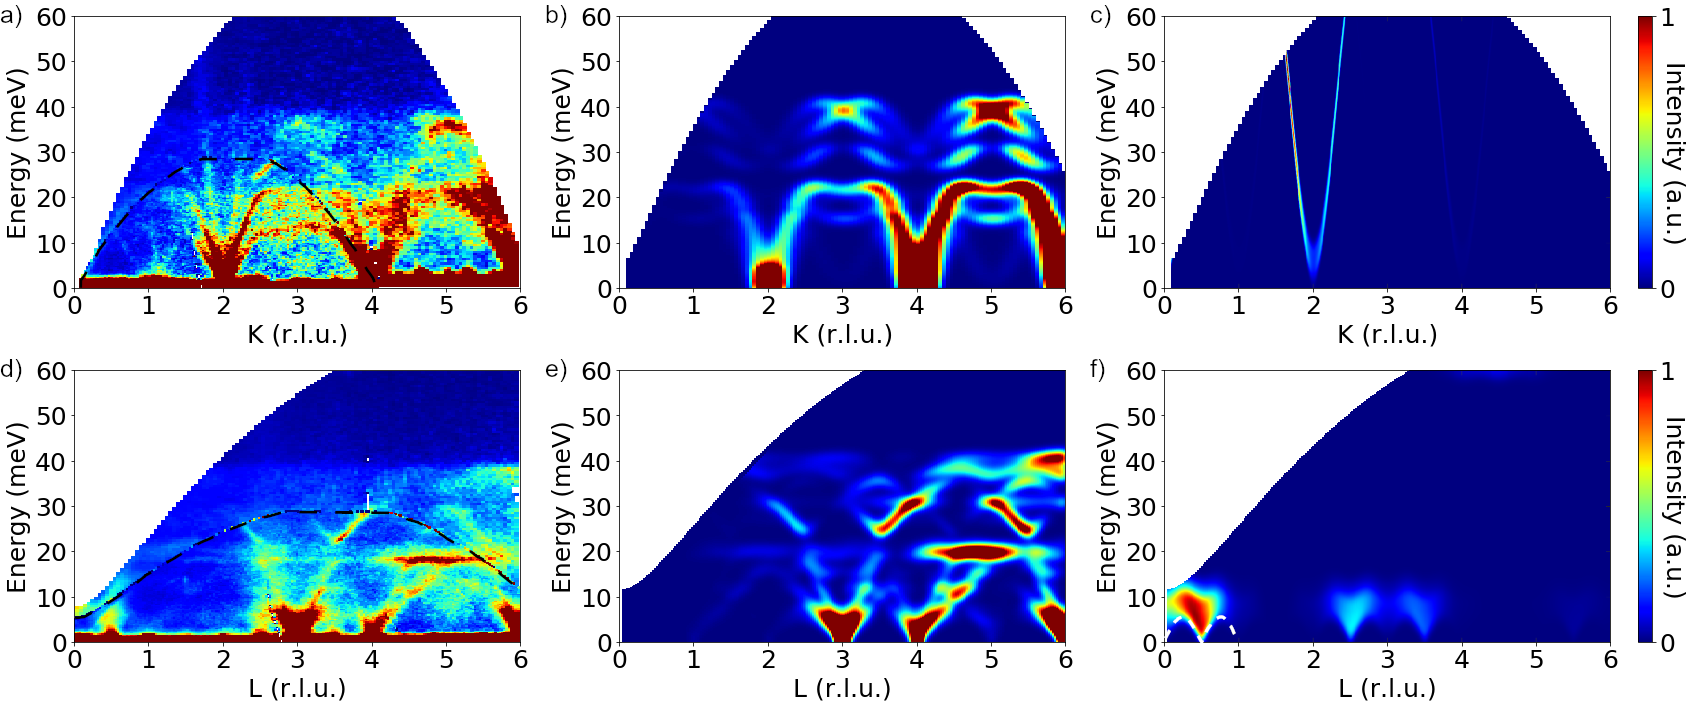
\includegraphics[width=\columnwidth]{figures/ch8/phonon_spectra_magnon_spectra_combined.png} \\
\caption{\label{fig:phonon_magnon_spectra}
Electronic band structure
}
\end{figure}

\begin{figure}
\centering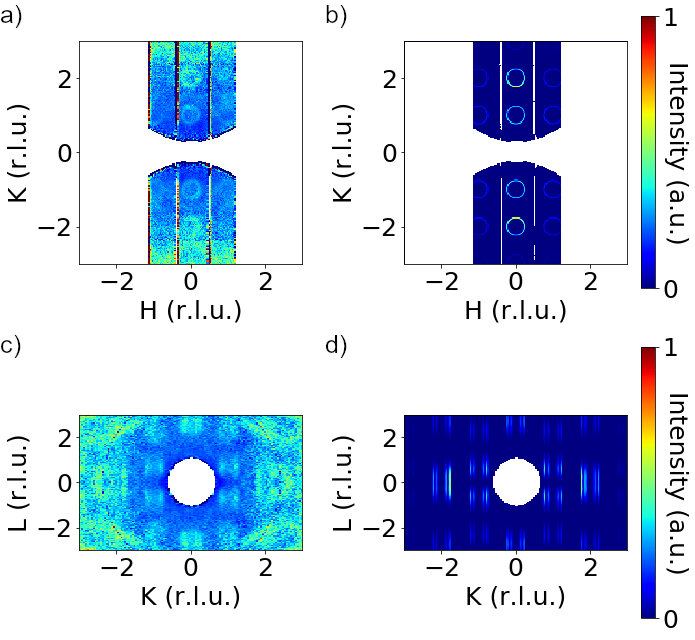
\includegraphics[width=\columnwidth]{figures/ch8/constant_energy_slices.png} \\
\caption{\label{fig:constant_energy_slices}
Electronic band structure
}
\end{figure}

\begin{figure}
\centering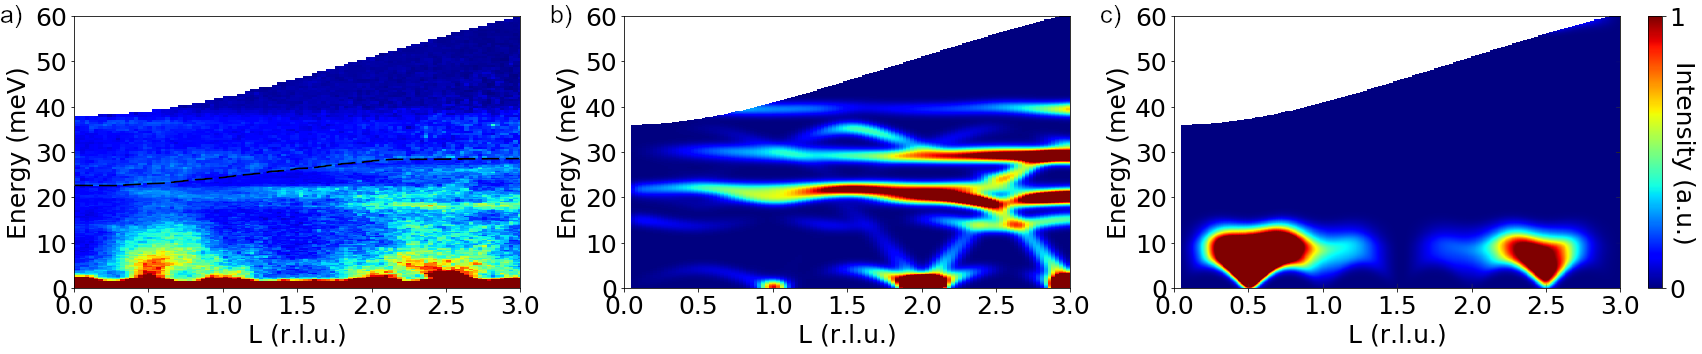
\includegraphics[width=\columnwidth]{figures/ch8/suppl_01L_INS_data.png} \\
\caption{\label{fig:01L_spectra}
Electronic band structure
}
\end{figure}

\begin{figure}
\centering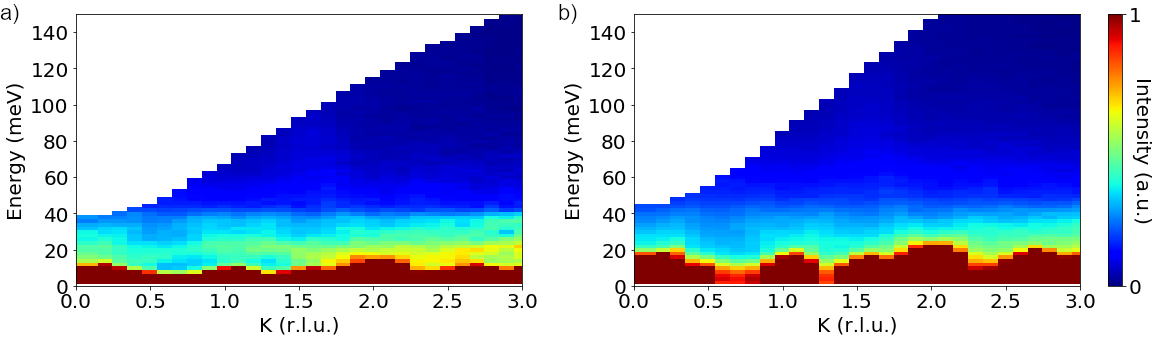
\includegraphics[width=\columnwidth]{figures/ch8/suppl_high_energy_data.png} \\
\caption{\label{fig:high_energy_data}
Electronic band structure
}
\end{figure}

\begin{figure}
\centering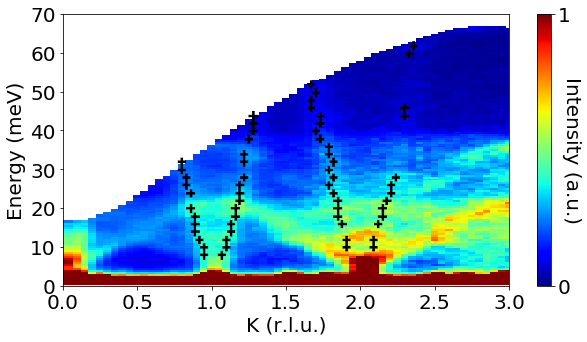
\includegraphics[width=\columnwidth]{figures/ch8/exp_data_points_0K0dot5.png} \\
\caption{\label{fig:exp_points}
Electronic band structure
}
\end{figure}

\begin{figure}
\centering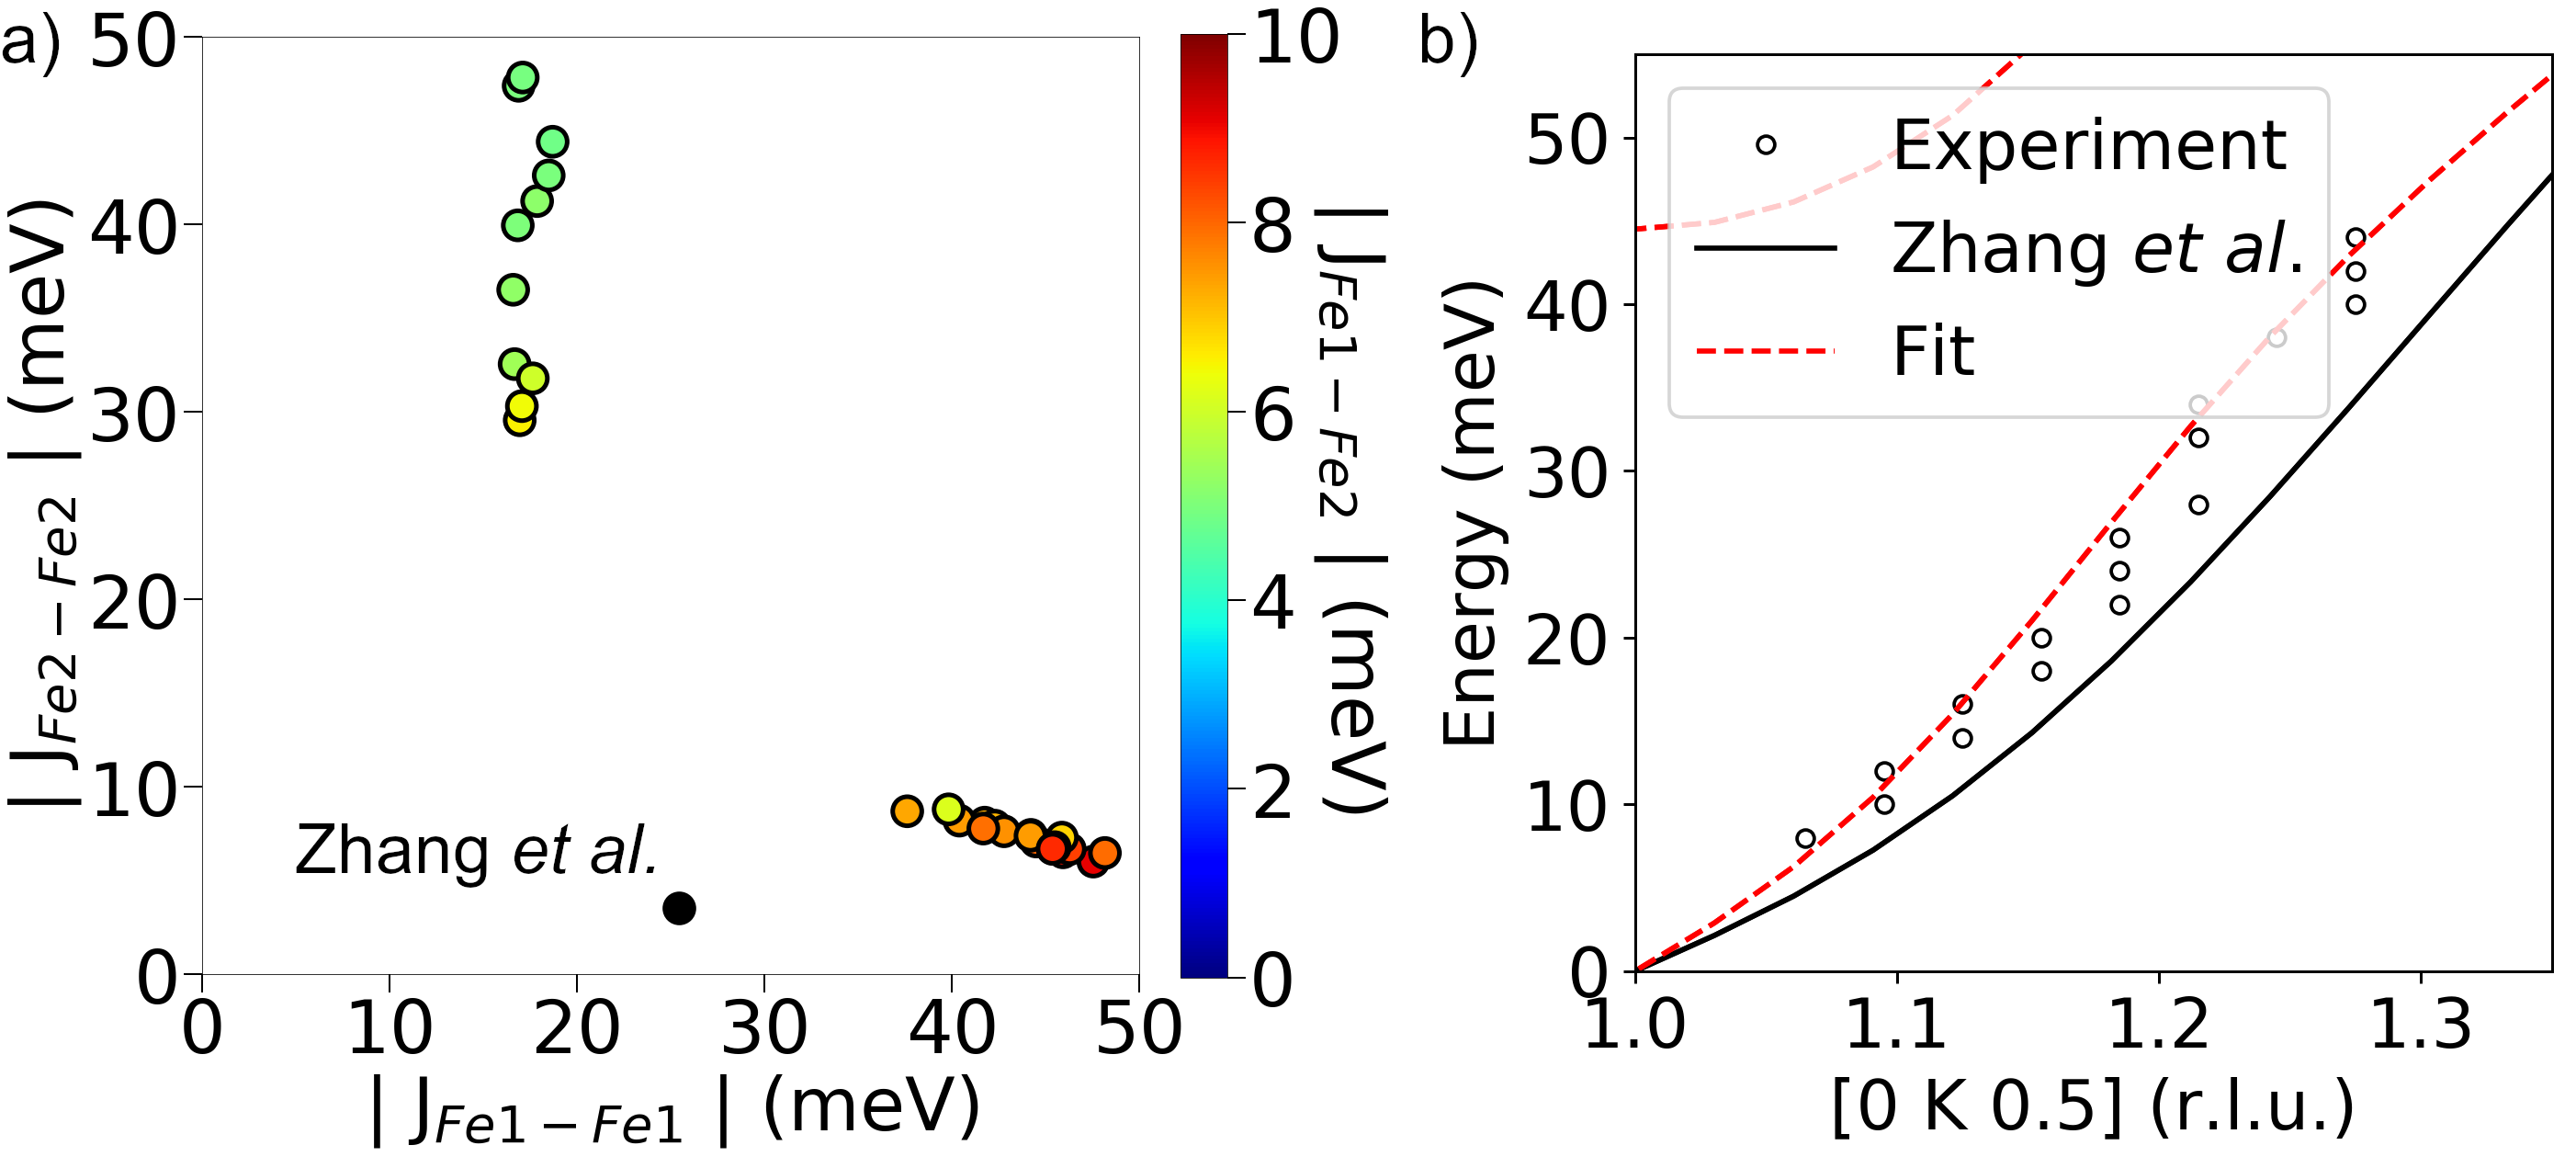
\includegraphics[width=\columnwidth]{figures/ch8/magnon_spectra_refinement.png} \\
\caption{\label{fig:refinement}
Electronic band structure
}
\end{figure}

\begin{figure}
\centering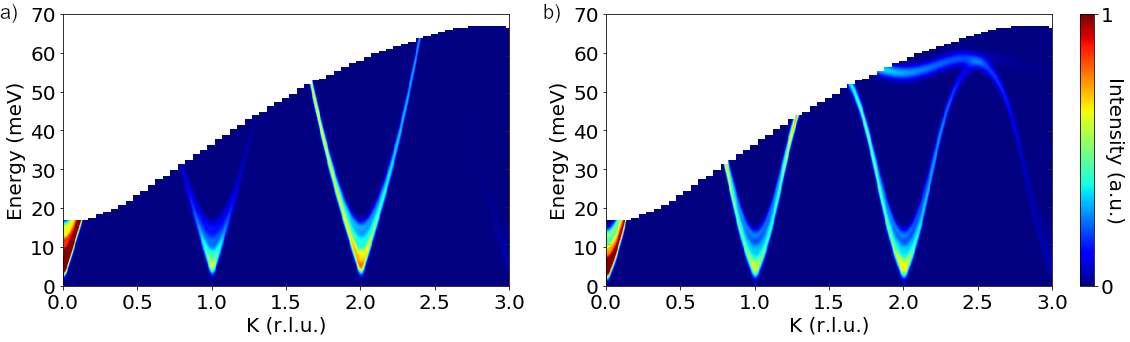
\includegraphics[width=\columnwidth]{figures/ch8/suppl_simulated_magnon_spectra_3J.png} \\
\caption{\label{fig:3J_fits}
Electronic band structure
}
\end{figure}

\Blindtext[6]

%chapter 9
\chapter{Conclusions}

\Blindtext[6]

\end{mainmatter}

% }}}

% {{{ back matter

\begin{backmatter}

\bibliographystyle{ieeetr}
\bibliography{thesis}

\end{backmatter}

%\appendix
%\chapter{My Appendix}

%\Blindtext[6]

% }}}

\end{document}
